\documentclass[12pt,twoside]{mit-template/mitthesis}

\usepackage{graphicx}
\usepackage[adobe-utopia]{mathdesign}
\usepackage{graphviz}
\usepackage{url}
\usepackage{amsmath}

% Remove footnote counter reset
\usepackage{remreset}
\makeatletter\@removefromreset{footnote}{chapter}\makeatother

% Enable hyper links inside the document
\usepackage[colorlinks=true,
linkcolor=black,
citecolor=black,
urlcolor=black]{hyperref}

\pagestyle{plain}

% Image directories
\graphicspath{{./depthcolor/img/}{./system/img/}{./applications/img/}{./performance/img/}}

% My system's classes
\newcommand{\ImageBuffer}{\texttt{Im\-age\-Buff\-er}}
\newcommand{\ImageBufferDepth}{\texttt{Im\-age\-Buff\-er.\-Depth}}
\newcommand{\ImageBufferColorModel}{\texttt{Im\-age\-Buff\-er.Col\-or\-Mod\-el}}
\newcommand{\Camera}{\texttt{Cam\-er\-a}}
\newcommand{\CameraReceiver}{\texttt{Cam\-er\-a\-Re\-ceiv\-er}}
\newcommand{\CameraData}{\texttt{Cam\-er\-a\-Da\-ta}}
\newcommand{\ColorCam}{\texttt{Col\-or\-Cam}}
\newcommand{\ColorCamData}{\texttt{Col\-or\-Cam\-Da\-ta}}
\newcommand{\ColorReceiver}{\texttt{Col\-or\-Re\-ceiv\-er}}
\newcommand{\ColorPacketHandler}{\texttt{Col\-or\-Pack\-et\-Han\-dler}}
\newcommand{\DCJavaAcquire}{\texttt{DC1394\-Ja\-va\-Ac\-quire}}
\newcommand{\SwissRangerCam}{\texttt{Swiss\-Rang\-er\-Cam}}
\newcommand{\SwissRangerCamData}{\texttt{Swiss\-Rang\-er\-Cam\-Da\-ta}}
\newcommand{\SwissRangerReceiver}{\texttt{Swiss\-Rang\-er\-Re\-ceiv\-er}}
\newcommand{\SwissRangerPacketHandler}{\texttt{Swiss\-Rang\-er\-Pack\-et\-Han\-dler}}
\newcommand{\SwissRangerJavaAcquire}{\texttt{Swiss\-Rang\-er\-Ja\-va\-Ac\-quire}}
\newcommand{\CalibrationTool}{\texttt{Cal\-i\-bra\-tion\-Tool}}
\newcommand{\CameraParameters}{\texttt{Cam\-er\-a\-Pa\-ram\-e\-ters}}
\newcommand{\ImageStream}{\texttt{Im\-age\-Stream}}
\newcommand{\Stream}{\texttt{Stream}}
\newcommand{\PacketOrganizer}{\texttt{Pack\-et\-Or\-gan\-iz\-er}}
\newcommand{\DepthColorCam}{\texttt{Depth\-Col\-or\-Cam}}
\newcommand{\DepthColorCalibrationTool}{\texttt{Depth\-Col\-or\-Cal\-i\-bra\-tion\-Tool}}
\newcommand{\DepthColorFusion}{\texttt{Depth\-Col\-or\-Fu\-sion}}
\newcommand{\FaceTracker}{\texttt{Face\-Track\-er}}
\newcommand{\FaceStream}{\texttt{Face\-Stream}}
\newcommand{\Face}{\texttt{Face}}
\newcommand{\KinectCam}{\texttt{Ki\-nect\-Cam}}
\newcommand{\KinectReceiver}{\texttt{Ki\-nect\-Re\-ceiv\-er}}
\newcommand{\KinectPacketHandler}{\texttt{Ki\-nect\-Pack\-et\-Han\-dler}}
\newcommand{\KinectJavaAcquire}{\texttt{Ki\-nect\-Ja\-va\-Ac\-quire}}
\newcommand{\KinectSkeleton}{\texttt{Ki\-nect\-Skel\-e\-ton}}
\newcommand{\KinectSkeletonStream}{\texttt{Ki\-nect\-Skel\-e\-ton\-Stream}}

% r1d1's classes
\newcommand{\RD}{\texttt{r1d1}}
\newcommand{\iUpdateable}{\texttt{iUp\-date\-a\-ble}}
\newcommand{\ImageView}{\texttt{Im\-age\-View}}
\newcommand{\DataProvider}{\texttt{Da\-ta\-Pro\-vid\-er}}
\newcommand{\DataHandler}{\texttt{Da\-ta\-Han\-dler}}
\newcommand{\SafePacketHandler}{\texttt{Safe\-Pack\-et\-Han\-dler}}
\newcommand{\iDataRecordHandler}{\texttt{iDa\-ta\-Re\-cord\-Han\-dler}}
\newcommand{\iDataRecord}{\texttt{iDa\-ta\-Re\-cord}}
\newcommand{\ByteBuffer}{\texttt{ja\-va.\-nio.\-Byte\-Buff\-er}}
\newcommand{\List}{\texttt{ja\-va.\-util.\-List}}

\begin{document}

% -*-latex-*-
% $Log: cover.tex,v $
% Revision 1.8  2008/05/13 15:02:15  jdreed
% Degree month is June, not May.  Added note about prevdegrees.
% Arthur Smith's title updated
%
% Revision 1.7  2001/02/08 18:53:16  boojum
% changed some \newpages to \cleardoublepages
%
% Revision 1.6  1999/10/21 14:49:31  boojum
% changed comment referring to documentstyle
%
% Revision 1.5  1999/10/21 14:39:04  boojum
% *** empty log message ***
%
% Revision 1.4  1997/04/18  17:54:10  othomas
% added page numbers on abstract and cover, and made 1 abstract
% page the default rather than 2.  (anne hunter tells me this
% is the new institute standard.)
%
% Revision 1.4  1997/04/18  17:54:10  othomas
% added page numbers on abstract and cover, and made 1 abstract
% page the default rather than 2.  (anne hunter tells me this
% is the new institute standard.)
%
% Revision 1.3  93/05/17  17:06:29  starflt
% Added acknowledgements section (suggested by tompalka)
% 
% Revision 1.2  92/04/22  13:13:13  epeisach
% Fixes for 1991 course 6 requirements
% Phrase "and to grant others the right to do so" has been added to 
% permission clause
% Second copy of abstract is not counted as separate pages so numbering works
% out
% 
% Revision 1.1  92/04/22  13:08:20  epeisach

% NOTE:
% These templates make an effort to conform to the MIT Thesis specifications,
% however the specifications can change.  We recommend that you verify the
% layout of your title page with your thesis advisor and/or the MIT 
% Libraries before printing your final copy.
\title{Integrated Vision Framework for a Robotics Research and Development Platform}

\author{Juli\'{a}n Hern\'{a}ndez Mu\~{n}oz}
% If you wish to list your previous degrees on the cover page, use the 
% previous degrees command:
       \prevdegrees{B.S. in Computer Science and Engineering \\ 
       		Massachusetts Institute of Technology (2009)}
% You can use the \\ command to list multiple previous degrees
%       \prevdegrees{B.S., University of California (1978) \\
%                    S.M., Massachusetts Institute of Technology (1981)}
\department{Department of Electrical Engineering and Computer Science}

% If the thesis is for two degrees simultaneously, list them both
% separated by \and like this:
% \degree{Doctor of Philosophy \and Master of Science}
\degree{Master of Engineering in Electrical Engineering and Computer Science}

% As of the 2007-08 academic year, valid degree months are September, 
% February, or June.  The default is June.
\degreemonth{June}
\degreeyear{2011}
\thesisdate{May 20, 2011}

%% By default, the thesis will be copyrighted to MIT.  If you need to copyright
%% the thesis to yourself, just specify the `vi' documentclass option.  If for
%% some reason you want to exactly specify the copyright notice text, you can
%% use the \copyrightnoticetext command.  
%\copyrightnoticetext{\copyright IBM, 1990.  Do not open till Xmas.}

% If there is more than one supervisor, use the \supervisor command
% once for each.
\supervisor{Dr. Cynthia Breazeal}{Associate Professor of Media Arts and Sciences}

% This is the department committee chairman, not the thesis committee
% chairman.  You should replace this with your Department's Committee
% Chairman.
\chairman{Dr. Christopher J. Terman}{Chairman, Masters of Engineering Thesis Committee}

% Make the titlepage based on the above information.  If you need
% something special and can't use the standard form, you can specify
% the exact text of the titlepage yourself.  Put it in a titlepage
% environment and leave blank lines where you want vertical space.
% The spaces will be adjusted to fill the entire page.  The dotted
% lines for the signatures are made with the \signature command.
\maketitle

% The abstractpage environment sets up everything on the page except
% the text itself.  The title and other header material are put at the
% top of the page, and the supervisors are listed at the bottom.  A
% new page is begun both before and after.  Of course, an abstract may
% be more than one page itself.  If you need more control over the
% format of the page, you can use the abstract environment, which puts
% the word "Abstract" at the beginning and single spaces its text.

%% You can either \input (*not* \include) your abstract file, or you can put
%% the text of the abstract directly between the \begin{abstractpage} and
%% \end{abstractpage} commands.

% First copy: start a new page, and save the page number.
\cleardoublepage
% Uncomment the next line if you do NOT want a page number on your
% abstract and acknowledgments pages.
% \pagestyle{empty}
\setcounter{savepage}{\thepage}
\begin{abstractpage}
%% The text of your abstract and nothing else (other than comments) goes here.
%% It will be single-spaced and the rest of the text that is supposed to go on
%% the abstract page will be generated by the abstractpage environment.  This
%% file should be \input (not \include 'd) from cover.tex.


This thesis presents the design of a vision framework integrated into a robotics research and development 
platform. The vision system was implemented as part of the software platform developed by the Personal 
Robots Group at the MIT Media Lab. Featuring representations for images and camera sensors, this system 
provides a structure that is used to build robot vision applications. One application shows how to merge the 
representations of two different cameras in order to create a camera entity that provides images with fused 
depth-color data. The system also allows the integration of computer vision algorithms that can be used
to extract perceptual information from the robot's surroundings. Two more applications show detection and 
tracking of human face and body pose using depth-color images.
\end{abstractpage}

% Additional copy: start a new page, and reset the page number.  This way,
% the second copy of the abstract is not counted as separate pages.
% Uncomment the next 6 lines if you need two copies of the abstract
% page.
% \setcounter{page}{\thesavepage}
% \begin{abstractpage}
% %% The text of your abstract and nothing else (other than comments) goes here.
%% It will be single-spaced and the rest of the text that is supposed to go on
%% the abstract page will be generated by the abstractpage environment.  This
%% file should be \input (not \include 'd) from cover.tex.


This thesis presents the design of a vision framework integrated into a robotics research and development 
platform. The vision system was implemented as part of the software platform developed by the Personal 
Robots Group at the MIT Media Lab. Featuring representations for images and camera sensors, this system 
provides a structure that is used to build robot vision applications. One application shows how to merge the 
representations of two different cameras in order to create a camera entity that provides images with fused 
depth-color data. The system also allows the integration of computer vision algorithms that can be used
to extract perceptual information from the robot's surroundings. Two more applications show detection and 
tracking of human face and body pose using depth-color images.
% \end{abstractpage}

\cleardoublepage

\section*{Acknowledgments}

I would like to start by thanking Dr. Cynthia Breazeal for giving me the opportunity of being part of the Personal 
Robots Group and for guiding me through the completion of this thesis.  Almost fifteen years ago I read a 
newspaper article about Kismet and her, and it inspired me to venture into the field of engineering.  It has been 
an honor working with her on this project.

I would also like to thank Philipp Robbel and Siggi Adalgeirsson, who have helped me from the moment I 
started at the group.  To Philipp, for taking me as his UROP and advising me in early projects.  To Siggi, for 
always lending a hand whenever I needed it.

Thanks to Dr. Peter Szolovits, my longtime academic advisor, for his support and mentoring throughout my 
bachelors and masters. I would also like to thank Dr. Berthold K.P. Horn and Dr. Antonio Torralba for sparking 
my interests in computer vision.

Thanks to my parents, Omar and Arzoris, for always being a source of great inspiration and for their constant 
motivation to strive for excellence.  To my brother and sister, Javier Arturo and Arzoris Marian, for giving me the 
support that only they can provide.

Finally, I would like to thank the Institute for six rewarding years. Getting an education from MIT is indeed like 
taking a drink from a fire hose.


%%%%%%%%%%%%%%%%%%%%%%%%%%%%%%%%%%%%%%%%%%%%%%%%%%%%%%%%%%%%%%%%%%%%%%
% -*-latex-*-
\pagestyle{plain}
  % -*- Mode:TeX -*-
%% This file simply contains the commands that actually generate the table of
%% contents and lists of figures and tables.  You can omit any or all of
%% these files by simply taking out the appropriate command.  For more
%% information on these files, see appendix C.3.3 of the LaTeX manual. 
\tableofcontents
\newpage
\listoffigures
\newpage
\listoftables



\chapter{Introduction} \label{introduction}

Robotics is a fast-growing field in academia, industry, and open-source communities, with many universities 
and corporations joining efforts in order to create frameworks that promote and advance the development of 
robotic systems. These systems are usually composed of both hardware and software platforms. As the field 
moves forward, it becomes necessary to describe the components that these platforms should have.

A vision framework is required by any system that needs to acquire, handle, and process images from 
cameras. In the same way cameras are typical sensors in robots, a vision framework should be a common 
component in any robotics software platform. Color cameras, for example, are widely available and the primary 
choice for the ``eyes'' of a robot. Other types of cameras, like depth cameras, are becoming cheaper and more 
accessible. 

This thesis provides a technical description of the vision system integrated into \RD{}, the Java software
platform developed and used by the Personal Robots Group at the MIT Media Lab. The \RD{} platform defines 
a cognitive architecture for interactive agents that allows designing real-time interactions between robots and 
persons. It features, among other things, flexible real-time integration of multiple perceptual inputs.

With this vision system, \RD{} applications have access to flexible image and camera representations. The 
image representation abstracts the source of the image, while the camera representations abstract the process 
of image acquisition. The modularity of these entities allows building applications without worrying about writing
code to interface with the cameras. This system is introduced in Chapter \ref{system}. 

Furthermore, the vision system lets the user define new representations by possibly combining existing ones.
Chapter \ref{depthcolor} explores how to fuse the data captured from two different types of 
cameras by merging their representations. The goal is to combine 2-dimensional information from a color 
camera with 3-dimensional information from a depth camera in order to produce fused depth-color images.

The motivation for merging these two sensors comes from the camera setup found in the second generation 
of the MDS robotic platform developed by the Personal Robots Group. The MDS is a humanoid robot that 
combines mobility, dexterity, and social interaction abilities \cite{MDS}. In its head, the MDS has a color camera
and a depth camera, both positioned in the forehead one below the other. 

The vision framework also integrates computer vision algorithms that can be used to gain perceptual 
information from the robot's surroundings. Chapter \ref{applications} presents face and body tracking 
capabilities that work on top of the image and camera representations. These algorithms serve to exemplify
the potential of the proposed vision system.

Although the framework is described as part of \RD{}, its design is meant to be modular and non-platform 
dependent. Most of the direct dependencies with other \RD{}'s components occur to take advantage of the 
intra-application communication system built into \RD{}. In general, the core concepts in the design of this vision 
system can be extracted and implemented in other research and development platforms. 
\chapter{Integrated Vision System} \label{system}

This chapter presents an integrated vision system for the \RD{} robotics research and development platform.
The proposed system introduces new representations for images and cameras in the \RD{} environment with 
designs that prove to be modular and flexible. In this system, not only images can vary in size, pixel depth, 
and color model, but they can be easily manipulated both within and outside \RD{} through applications with 
access to the native system memory.

Moreover, this system presents a core structure for a camera that can be replicated into different camera
types, including, as shown in this chapter, a color camera and a 3D time-of-flight camera. These
representations are flexible enough to allow a camera be either a device directly connected to the computer 
running \RD{}, or a device connected remotely that transfers the image data through the network.

Section \ref{imagebuffer} of this chapter discusses the image representation in the integrated vision system, 
while Sections \ref{camera} and \ref{camerareceiver} discuss the base camera representation. 
Sections \ref{colorcam} and \ref{swissrangercam} show the flexibility of the system by presenting the 
implementations for two types of cameras. Finally, the last three sections of the chapter, Sections 
\ref{calibrationtool}, \ref{imagestream}, and \ref{packetorganizer}, further discuss some of the entities used in
the cameras' implementations.

\section{Image Buffer} \label{imagebuffer}
The \ImageBuffer{} class represents an image in the \RD{} environment. An instance of this class is defined 
by four fields. The first three are the image's width, height, and pixel depth. The fourth field can be either
the image's color model or its number of channels.\footnote{Not all images require a color model. An 
example is the depth image acquired by a range sensor.} 
The different possible combinations of values for these fields allow a flexible description of an image inside
the programming environment. Tables \ref{imagebufferdepth} and \ref{imagebuffercolormodel} show the 
available values for the depth and color model fields, as described by the \ImageBufferDepth{} and 
\ImageBufferColorModel{} enum types.

\begin{table}[ht]
\caption{Pixel depth values in the \ImageBufferDepth{} enum}
\begin{center}
\begin{tabular}{| l | l |}
	\multicolumn{2}{c}{\ImageBufferDepth{}} \\
	\hline 
	Depth 			& Description \\
	\hline \hline
	\texttt{BYTE} 		& Unsigned 8-bit integer \\
	\texttt{SHORT}	 	& Unsigned 16-bit integer \\
	\texttt{FLOAT}	 	& 32-bit floating-point single precision \\
	\texttt{DOUBLE} 	& 64-bit floating-point double-precision \\
	\hline
\end{tabular}
\end{center}
\label{imagebufferdepth}
\end{table}

\begin{table}[ht]
\caption{Color model values in the \ImageBufferColorModel{} enum}
\begin{center}
\begin{tabular}{| l | l |}
	\multicolumn{2}{c}{\ImageBufferColorModel{}} \\
	\hline 
	Color Model 		& Description \\
	\hline \hline
	\texttt{BGR} 		& Blue-Green-Red channels \\
	\texttt{BGRA} 		& Blue-Green-Red-Alpha channels \\
	\texttt{RGB}	 	& Red-Green-Blue channels \\
	\texttt{RGBA}	 	& Red-Green-Blue-Alpha channels \\
	\texttt{GRAY}	 	& Grayscale channel \\
	\hline
\end{tabular}
\end{center}
\label{imagebuffercolormodel}
\end{table}

In an image buffer, the image data is stored in an underlying \ByteBuffer{} object. 
Part of the flexibility of the \ImageBuffer{} class is attributed to the versatility of a byte buffer with
respect to the data it can hold. Furthermore, the byte buffer within an image buffer is created to be 
direct. A direct byte buffer in Java allocates its space in native system memory, outside of the Java 
virtual machine's memory heap. This allows other programs outside Java to use native code to access
the same allocated memory space. An example of the advantage of using direct buffers is the 
implementation of an interface between \RD{} and the OpenCV computer vision open source library.
This interface enables performing OpenCV functions directly onto the Java images through native code.

Pixels in an image buffer are stored row by row with interleaved channels, starting at the top-left pixel. 
The methods to access and manipulate the image data are specific to the image's pixel depth. For 
example, the methods of the form \texttt{get\-Byte\-Pix\-el} are used to access pixels in an image of depth 
\texttt{BYTE}. The different versions of the same getter method trade off convenience for performance. 
Getter methods that accept an array as input speed up a loop through the image's pixels by
avoiding the overhead of creating the output array on every call.


\section{Camera} \label{camera}
The \Camera{} abstract class is the base representation of a camera in the \RD{} environment.  As listed in 
Table \ref{cameramethods}, this class defines methods to access information about a camera 
(\texttt{get\-Width}, \texttt{get\-Height}, \texttt{get\-Time\-stamp}, \texttt{get\-Frame\-Rate}), methods to capture 
images from the camera (\texttt{start\-Cap\-turing}, \texttt{grab\-Im\-age}), and methods to perform camera 
calibration (\texttt{start\-Cal\-i\-bra\-tion}). 

\begin{table}[ht]
\caption{Public methods in the \Camera{} class}
\begin{center}
\begin{tabular}{| l |}
	\hline 
	\multicolumn{1}{| c |}{\Camera{}} \\
	\hline \hline
	\texttt{startCapturing} \\
	\texttt{startCalibration} \\
	\texttt{grabImage}	\\
	\texttt{getWidth} \\
	\texttt{getHeight} \\
	\texttt{getTimestamp} \\
	\texttt{getFrameRate} \\
	\hline
\end{tabular}
\end{center}
\label{cameramethods}
\end{table}

By providing an abstract implementation, the \Camera{} class lets its subclasses describe different types of 
cameras while specifying a common structure for them.  In this framework, \ColorCam{} and 
\SwissRangerCam{} are the main examples of extending the \Camera{} class to represent 
cameras that capture different types of data: the first one represents a conventional color camera while 
the second one represents a 3D time-of-flight camera (see Sections \ref{colorcam} and \ref{swissrangercam}). 
This design allows a flexible definition of what a camera is and lets the user choose the representation 
of the data captured by a specific sensor.

Furthermore, an object of type \Camera{} is a subtype of \DataProvider{}. A data provider is an object that 
can publish user defined datatypes in \RD{}'s  intra-application communication system, allowing other objects 
called data handlers to subscribe to and receive the provided data. In the case of a \Camera{} object, 
the provided data is represented by the abstract class \CameraData{}. Subclasses of \CameraData{}
define the datatypes captured by different camera sensors. For example, \ColorCamData{} and 
\SwissRangerCamData{} represent the data provided by \ColorCam{} and \SwissRangerCam{}, respectively.

\section{Camera Receiver} \label{camerareceiver}
The \CameraReceiver{} abstract class defines the base structure of the mechanism that will acquire and handle
data from the camera sensors. It implements two \RD{} interfaces. The first one is the \iUpdateable{} interface,
which describes classes that have an \texttt{up\-date} method. The main loop of an \RD{} application calls 
\texttt{up\-date} on all the objects that have been registered as updatable. For the camera receiver this means 
that the \texttt{up\-date} method can be used to grab an image from a camera on every loop.

The second interface used by the \CameraReceiver{} class is the \iDataRecordHandler{}. This interface is part
of \RD{}'s intra-application communication system. It is used to define a class that can handle \iDataRecord{} 
objects being sent from another application. A class that implements this interface has a 
\texttt{han\-dle\-Da\-ta\-Re\-cord} method that handles the incoming data record objects. The camera receiver
can use this method to receive records containing image data.

Table \ref{camerareceivermethods} lists the two abstract methods declared in the \CameraReceiver{} class.
These methods are used to start the image receiving process and query the receiver if it has image data 
available to be accessed or retrieved. 

\begin{table}[ht]
\caption{Public methods in the \CameraReceiver{} class }
\begin{center}
\begin{tabular}{| l |}
	\hline 
	\multicolumn{1}{| c |}{\CameraReceiver{}} \\
	\hline \hline
	\texttt{startReceiving} \\
	\texttt{isDataAvailable} \\
	\hline
\end{tabular}
\end{center}
\label{camerareceivermethods}
\end{table}
	
\section{Color Camera} \label{colorcam}
The \ColorCam{} class extends \Camera{} to represent a color camera. In the \RD{} environment, a color
camera can be a camera sensor connected directly to the computer running the system, or a camera sensor
connected to some other device that sends the images over the network to \RD{}. This versatility is provided 
by \ColorCam{} through the \ColorReceiver{} class. While the color receiver is in charge of acquiring and 
handling the images from the camera, a color camera provides access to the image buffer, the image view, 
and the camera calibration tool. Additionally, it provides the implementation of all abstract methods defined 
by the \Camera{} class. Table \ref{colorcammethods} lists the methods that a color camera adds to the 
base camera representation.

\begin{table}[ht]
\caption{Public methods in the \ColorCam{} class}
\begin{center}
\begin{tabular}{| l |}
	\hline 
	\multicolumn{1}{| c |}{\ColorCam{}} \\
	\multicolumn{1}{| c |}{{\small \texttt{extends} \Camera{}}} \\
	\hline \hline
	\texttt{getImage} \\
	\texttt{getImageView} \\
	\texttt{getCalibrationTool} \\
	\hline
\end{tabular}
\end{center}
\label{colorcammethods}
\end{table}

There are two ways of accessing the camera's images. One way is through the \ColorCam{} object's internal 
image buffer, which stores a copy of the last grabbed image. This image buffer is obtained by calling the
\texttt{get\-Im\-age} method. The second way takes advantage of \RD{}'s intra-application communication 
system and consists of subscribing to the data objects of type \ColorCamData{} through the \DataHandler{} 
interface. The \texttt{han\-dle\-Da\-ta} method of the data handler receives the data objects that contain an 
image buffer with the copy of the grabbed image.

Therefore, every time a call to \texttt{grab\-Im\-age} returns successfully (i.e. returns a \texttt{true} value) two 
things happen: (1) the acquired image is stored in the internal image buffer and (2) it is published through the 
\DataProvider{} interface. Accessing the images from the image buffer gives the user more precision when it
is necessary to process the image right after it is grabbed. Receiving a published image contains the 
overhead of going through the data dispatcher mechanism, but simplifies the communication between
\RD{} applications. 

The \ColorCam{} class adds a second version of the \texttt{grab\-Im\-age} method. This second version takes
as input a value that represents the desired timestamp for the grabbed image. This method is 
useful when synchronizing two or more cameras: given the timestamp of an image from one of the cameras
this \texttt{grab\-Im\-age} method can be used to retrieve the closest corresponding image from the other
cameras.  

A color camera also provides the option of displaying the image stream using \RD{}'s graphics display system.
This is achieved by instantiating an \ImageView{} object linked to the color camera's internal image buffer. 
Every time an image is acquired the image view needs to be refreshed in order to display the new data on the 
buffer. This image view is accessed by calling the \texttt{get\-Im\-age\-View} method.

Finally, the methods to perform camera calibration and retrieve the camera's parameters are available 
through the \CalibrationTool{} object that is associated with every instance of \ColorCam{}. Upon the creation
of the color camera, a calibration tool object is constructed and linked to the camera's internal image buffer. 
When the \texttt{start\-Cal\-i\-bra\-tion} method is called, the calibration tool is started. Then, the user can
use the methods in the calibration tool, obtained by calling the \texttt{get\-Cal\-i\-bra\-tion\-Tool} method, to 
calibrate the camera (see Section \ref{calibrationtool}). 

The following sections present and discuss the modules that compose the \ColorCam{} class. The 
module dependency diagram in Figure \ref{colorcammoduledependency} shows how these classes 
are related to each other. 

\begin{figure}[t]
\begin{center}
\digraph[scale=0.75]{ColorCam}{
	graph [rankdir = "TB" margin = 0];
	node [shape = "box" style = "filled" fillcolor = "gainsboro" fontsize = "12" fontname = "Courier"];
		Camera CameraReceiver CameraData Stream;
	node [shape = "box" style = "filled" fillcolor = "floralwhite" fontsize = "12" fontname = "Courier"];
	{ rank = "source"; CameraReceiver Camera CameraData Stream;}
	{ rank = "same"; ColorCam ColorCamData;}
	{ rank = "same"; ColorReceiver CalibrationTool;}
	{ rank = "same"; ColorPacketHandler DC1394JavaAcquire ImageStream;}
	{ rank = "sink"; PacketOrganizer;}
	edge [arrowhead = "normal"];
	Camera -> CameraData;
	ColorCam -> Camera [arrowhead = "empty"] ;
	ColorCam -> ColorCamData;
	ColorCam -> ColorReceiver ;
	ColorCam -> CalibrationTool;
	ColorCamData -> CameraData [arrowhead = "empty"];
	ColorReceiver -> CameraReceiver [arrowhead = "empty"];
	ColorReceiver -> ColorPacketHandler;
	ColorReceiver -> DC1394JavaAcquire;
	ColorReceiver -> ImageStream;
	ImageStream -> Stream [arrowhead = "empty"];
	ColorPacketHandler -> PacketOrganizer;
}
\caption[\ColorCam{}'s module dependency diagram]{\ColorCam{} module dependency diagram. Arcs with 
white arrows represent subtype relations (A $\vartriangleright$ B = A extends B) while arcs with black arrows 
represent implementation relations (A $\blacktriangleright$ B = A uses B). Gray rectangles represent abstract 
classes. The \ImageBuffer{} class is omitted from this diagram.}
\label{colorcammoduledependency}
\end{center}
\end{figure}



	
	\subsection{Color Receiver} \label{colorreceiver}
	The \ColorReceiver{} class extends \CameraReceiver{} to provide the mechanism that interfaces with a color 
camera. It allows the user to acquire images directly from a Firewire camera or to receive the color images via a 
network transfer. Image acquisition from the camera is achieved using the libdc1394 API, a library of functions to 
control Firewire cameras that conform to the 1394-based Digital Camera Specifications \cite{libdc1394}. The 
network transfer is achieved through IRCP, the network communication protocol used by \RD{} \cite{IRCP}.
Table \ref{colorreceivermethods} lists the methods that the \ColorReceiver{} class adds to the camera receiver 
representation.

\begin{table}[ht]
\caption{Public methods in the \ColorReceiver{} class }
\begin{center}
\begin{tabular}{| l |}
	\hline 
	\multicolumn{1}{| c |}{\ColorReceiver{}} \\
	\multicolumn{1}{| c |}{{\small \texttt{extends} \CameraReceiver{}}} \\
	\hline \hline
	\texttt{getImage} \\
	\texttt{handleDataRecord} \\
	\texttt{update} \\
	\hline
\end{tabular}
\end{center}
\label{colorreceivermethods}
\end{table}

Upon initialization, the color receiver first tries to connect to a Firewire camera. The \texttt{up\-date} method
is in charge of acquiring the images using the \DCJavaAcquire{} methods. If the color receiver does not find a 
camera or if it fails when attempting to connect to one, it will proceed to start the IRCP network connection by 
setting up a \ColorPacketHandler{} (the user has the option of forcing this network connection). As discussed in 
Section \ref{camerareceiver}, the images received by the packet handler are sent to the color receiver through 
the \iDataRecordHandler{} interface. The color receiver calls the \texttt{han\-dle\-Da\-ta\-Re\-cord} method to 
handle the incoming data record objects.

The \ColorReceiver{} class is flexible with the type of image it can handle. The image type is specified by a 
set of public static variables that the user can modify. Table \ref{colorreceivervariables} contains the list of all 
the variables available to the user. When running on libdc1394 mode the user can change the size of the image 
captured from the camera. When running on network mode the user can modify the image size, pixel depth, and 
color model according to what is being transferred over the network. 

\begin{table}[ht]
\caption{User-modifiable static variables in the \ColorReceiver{} class}
\begin{center}
\begin{tabular}{| l | l |}
	\multicolumn{2}{c}{\ColorReceiver{}} \\
	\hline
	Variable & Description \\
	\hline \hline
	\texttt{WIDTH} 						& The image width \\
	\texttt{HEIGHT} 					& The image height \\
	\texttt{DEPTH} 						& The image pixel depth \\
	\texttt{COLOR\_MODEL} 				& The image color model \\
	\texttt{CAMERA\_GUID} 				& The camera GUID \\
	\texttt{DC1394\_FRAME\_RATE} 		& The camera capturing frame rate \\
	\texttt{DC1394\_ISO\_SPEED} 			& The camera ISO speed \\
	\texttt{UNDISTORT} 				& Flag to undistort the image \\
	\texttt{COMPRESSED\_IMAGE} 		& Flag if image is compressed \\
	\texttt{STREAM\_CAPACITY} 			& The receiver image stream size \\
	\texttt{VISION\_MINOR\_TYPE} 		& The IRCP minor type \\
	\texttt{PACKET\_HANDLER\_NAME} 	& The packet handler name \\
	\texttt{PACKET\_HANDLER\_KEY} 				& The packet handler key \\
	\hline
\end{tabular}
\end{center}
\label{colorreceivervariables}
\end{table}

Besides handling a real time image stream, the color receiver can store a user-defined number of last seen 
images in memory. The mechanism that processes the image stream works like a First-In-First-Out queue: 
fresh images are stored at the tail of the stream while old images are retrieved from the head of the stream. 
The size of the stream determines the number of images that can be saved in memory. This system allows
to synchronize two or more cameras by finding in their streams the images with matching (or closest) 
timestamp. The \ImageStream{} class contains the implementation of this mechanism (see Section 
\ref{imagestream}).

	\subsection{Color Packet Handler} \label{colorpackethandler}
	The \ColorPacketHandler{} class is a subtype of \SafePacketHandler{}, a class part of the receiving end in 
the IRCP communication system. The \ColorReceiver{} object creates a color packet handler to manage the 
packets sent over the network that correspond to image data from a color camera. Therefore, the color
packet handler needs to know how the color information is encoded in the incoming packet. 

In order to manage a large number of sent packets, some of which can get lost or arrive out of sequence, 
the color packet handler implementation uses a \PacketOrganizer{} object to organize the incoming 
data (see Section \ref{packetorganizer}). The packet organizer takes the received packets, which 
consist of subparts of the whole image, and informs the color packet handler once there are images ready
to be retrieved.

Table \ref{colorpackethandlermethods} contains the method that the color packet handler overrides 
from the safe packet handler class. 

\begin{table}[ht]
\caption{Public methods in the \ColorPacketHandler{}  class}
\begin{center}
\begin{tabular}{| l |}
	\hline 
	\multicolumn{1}{| c |}{\ColorPacketHandler{}} \\
	\multicolumn{1}{| c |}{{\small extends \SafePacketHandler{}}} \\
	\hline \hline
	\texttt{safeHandle} \\
	\hline
\end{tabular}
\end{center}
\label{colorpackethandlermethods}
\end{table}
	\subsection{DC1394 Java Acquire} \label{dc1394javaacquire}
	The \DCJavaAcquire{} class establishes the Java interface to the libdc1394 library. Since libdc1394 is 
written in C, this class uses the Java Native Interface (JNI) framework to access the library functions.
The native methods declared in the Java layer are implemented in a separate C layer, and this
implementation is packaged in the \RD{} JNI library called libdc1394\-Ja\-va\-Ac\-quire. 

The \DCJavaAcquire{} class simplifies the access to a Firewire camera by declaring the methods listed
in Table \ref{dcjavaacquiremethods}. The \texttt{get\-GUIDs} method returns a list of GUIDs from the 
available Firewire cameras, and \texttt{start\-Cap\-tur\-ing}, \texttt{stop\-Cap\-tur\-ing}, and \texttt{get\-Im\-age}
are used to control and acquire images from them. The last two methods in the list are specific to Firewire 
cameras produced by Point Grey, and they are used to convert captured grayscale images to color images.

\begin{table}[ht]
\caption{Public methods in the \DCJavaAcquire{} class}
\begin{center}
\begin{tabular}{| l |}
	\hline 
	\multicolumn{1}{| c |}{\DCJavaAcquire{}} \\
	\hline \hline
	\texttt{getGUIDs} \\
	\texttt{startCapturing} \\
	\texttt{stopCapturing} \\
	\texttt{getImage} \\
	\texttt{retrievePointGreyBayerTile} \\
	\texttt{convertPointGreyMonoToBGR} \\
	\hline
\end{tabular}
\end{center}
\label{dcjavaacquiremethods}
\end{table}
	
\section{SwissRanger Camera} \label{swissrangercam}
The \SwissRangerCam{} class and its components are very similar to the classes that describe a color 
camera in \RD{}. This proves that the system can represent cameras following a similar core structure. Like 
\ColorCam{}, the \SwissRangerCam{} class extends \Camera{}. In this case it represents a SwissRanger
sensor, a 3D time-of-flight camera produced by Mesa Imaging \cite{SR4000Manual}. The SwissRanger 
can capture depth information (z-coordinates) from a scene, as well as x-coordinates and y-coordinates for 
each of the depth points. Associated with this data is the amplitude and the confidence map, which provide
measurements of the quality of the acquired data. 

In the representation, the SwissRanger can be connected directly to the computer running the system, or it 
can be connected to some other device that sends the images over the network to \RD{}. This versatility is 
provided through the \SwissRangerReceiver{} class. While the SwissRanger receiver is in charge of acquiring 
and handling the images from the camera, the SwissRanger camera provides access to the image buffers, 
the image views, and the camera calibration tool, as well as the implementation of all abstract methods 
defined by the \Camera{} class. Furthermore, it contains the information about the modulation frequency 
on which the SwissRanger is running, and static methods to create visualizations for the depth and amplitude 
data. Table \ref{swissrangercammethods} lists the methods that the SwissRanger class adds to the base 
camera representation.

\begin{table}[ht]
\caption{Public methods in the \SwissRangerCam{} class}
\begin{center}
\begin{tabular}{| l |}
	\hline 
	\multicolumn{1}{| c |}{\SwissRangerCam{}} \\
	\multicolumn{1}{| c |}{{\small \texttt{extends} \Camera{}}} \\
	\hline \hline
	\texttt{getDepth} \\
	\texttt{getAmplitude} \\
	\texttt{getX} \\
	\texttt{getY} \\
	\texttt{getConfidenceMap} \\
	\texttt{getDepthDisplay} \\
	\texttt{getAmplitudeDisplay} \\
	\texttt{getDepthView} \\
	\texttt{getAmplitudeView} \\
	\texttt{getCalibrationTool} \\
	\texttt{getModulationFrequency} \\
	\texttt{createDisplays} \\
	\texttt{threshold} \\
	\texttt{toMeters} \\
	\hline
\end{tabular}
\end{center}
\label{swissrangercammethods}
\end{table}

There are two ways of accessing the image data captured by the SwissRanger. One way is through the 
camera object's internal image buffers, which store copies of the last grabbed images. The depth data
is obtained by calling the \texttt{get\-Depth} method, and the amplitude data is obtained by calling 
\texttt{get\-Am\-pli\-tude}. The x-coordinate, y-coordinate, and confidence map data are obtained by calling
\texttt{getX}, \texttt{getY}, and \texttt{get\-Con\-fi\-dence\-Map}, respectively.

The second way takes advantage of \RD{}'s intra-application communication system and consists of 
subscribing to the data objects of type \SwissRangerCamData{} through the \DataHandler{} interface. 
A SwissRanger data object contains the same number of image buffers as described before, each with a 
copy of the last grabbed image. The \texttt{han\-dle\-Da\-ta} method of the data handler receives these data 
objects. 

Similar to the \ColorCam{} class, when the \texttt{grab\-Im\-age} method returns successfully the acquired 
images are stored in the internal image buffers and then are published through the \DataProvider{} interface. 
Accessing the images directly from the image buffers avoids the overhead of going through the data 
dispatcher mechanism and allows the user to process the images right after they are grabbed. However, 
receiving the images published through the data dispatcher simplifies the communication between \RD{} 
applications. 

Furthermore, the \SwissRangerCam{} class also adds a second version of the \texttt{grab\-Im\-age} method.
The reason for this method becomes clearer now. A Firewire color camera could be synchronized with a 
SwissRanger, but differences in the devices and their capturing mechanisms might not give the user the 
same capturing frame rate nor the same timestamp for images captured at the same time. Since this second 
version of the \texttt{grab\-Im\-age} method takes as input a desired timestamp for the grabbed image, it is 
possible to get a timestamp from one of the cameras and retrieve the closest corresponding image from the 
second camera taking into account a timestamp offset.

The \SwissRangerCam{} class provides the option of displaying visualizations for the depth image stream 
and the amplitude image stream. The methods \texttt{get\-Depth\-Dis\-play} and 
\texttt{get\-Am\-pli\-tude\-Dis\-play} return image buffers with BGR color model and \texttt{BYTE} pixel depth 
containing the image data of the visualizations. These image buffers are linked to \ImageView{} objects and 
are obtained through the \texttt{get\-Depth\-View} and \texttt{get\-Am\-pli\-tudeView} methods. The method 
\texttt{cre\-ate\-Dis\-plays} is used to create the visualizations from the raw depth and amplitude data.

The \CalibrationTool{} class is again used to provide the methods that perform camera calibration and retrieve
the camera's parameters. Since the amplitude image is visually close to a grayscale image, the calibration tool 
object is linked to the internal amplitude image buffer of the \SwissRangerCam{} instance. The user can 
access this object through the \texttt{get\-Cal\-i\-bra\-tion\-Tool} method, and then calibrate the camera by 
using the methods discussed in Section \ref{calibrationtool}.

The following sections present and discuss the modules that make up the \SwissRangerCam{} class. Figure 
\ref{swissrangercammoduledependency} shows a module dependency diagram that indicates how these 
classes are related to each other. 

\begin{figure}[t]
\begin{center}
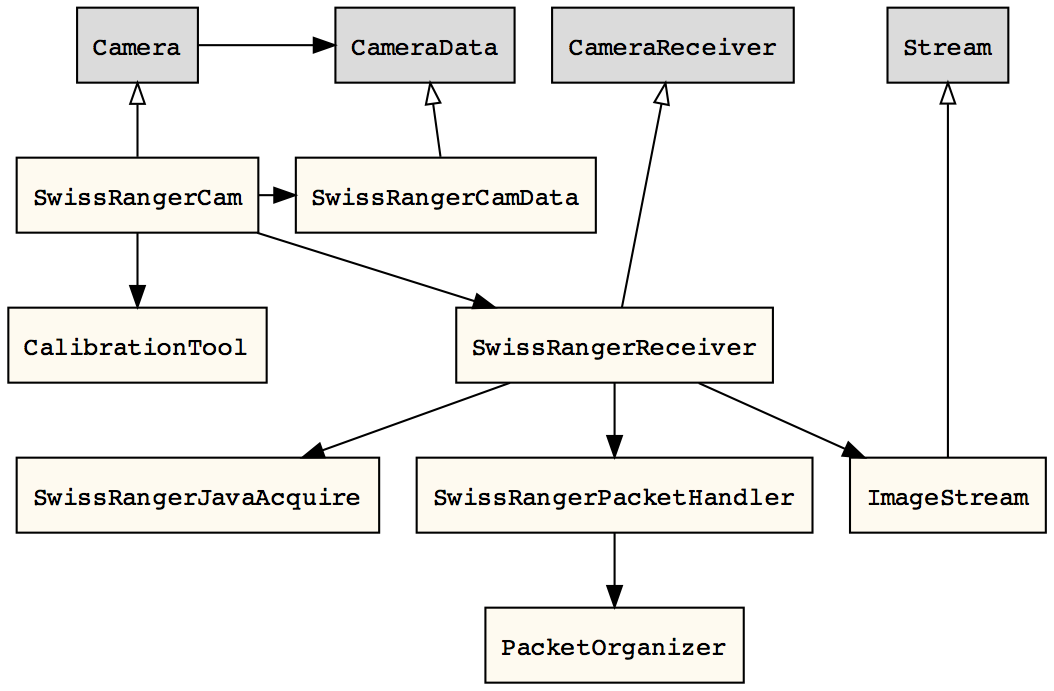
\includegraphics[width = 15cm]{SwissRangerCam.png}
%\digraph[scale=0.75]{SwissRangerCam}{
	graph [rankdir = "TB" margin = 0];
	node [shape = "box" style = "filled" fillcolor = "gainsboro" fontsize = "12" fontname = "Courier"];
		Camera CameraReceiver CameraData Stream;
	node [shape = "box" style = "filled" fillcolor = "floralwhite" fontsize = "12" fontname = "Courier"];
	{ rank = "source"; CameraReceiver Camera CameraData Stream;}
	{ rank = "same"; SwissRangerCam SwissRangerCamData;}
	{ rank = "same"; SwissRangerReceiver CalibrationTool;}
	{ rank = "same"; SwissRangerPacketHandler SwissRangerJavaAcquire ImageStream;}
	{ rank = "sink"; PacketOrganizer;}
	edge [arrowhead = "normal"];
	Camera -> CameraData;
	SwissRangerCam -> Camera [arrowhead = "empty"] ;
	SwissRangerCam -> SwissRangerCamData;
	SwissRangerCam -> SwissRangerReceiver ;
	SwissRangerCam -> CalibrationTool;
	SwissRangerCamData -> CameraData [arrowhead = "empty"];
	SwissRangerReceiver -> CameraReceiver [arrowhead = "empty"];
	SwissRangerReceiver -> SwissRangerPacketHandler;
	SwissRangerReceiver -> SwissRangerJavaAcquire;
	SwissRangerReceiver -> ImageStream;
	ImageStream -> Stream [arrowhead = "empty"];
	SwissRangerPacketHandler -> PacketOrganizer;
}
\caption[\SwissRangerCam{}'s module dependency diagram]{\SwissRangerCam{} module dependency 
diagram. Arcs with white arrows represent subtype relations (A $\vartriangleright$ B = A extends B) while 
arcs with black arrows represent implementation relations (A $\blacktriangleright$ B = A uses B). Gray 
rectangles represent abstract classes. The \ImageBuffer{} class is omitted from this diagram.}
\label{swissrangercammoduledependency}
\end{center}
\end{figure}

	
	\subsection{SwissRanger Receiver} \label{swissrangerreceiver}
	The \SwissRangerReceiver{} class extends \CameraReceiver{} to provide the mechanism that interfaces with a 
SwissRanger camera. It allows the user to acquire images directly from a SwissRanger or to receive depth, 
amplitude, x-coordinate, y-coordinate, and confidence images via a network transfer. Image acquisition from 
the camera is achieved using the SwissRanger driver API that is provided by Mesa Imaging. The network 
transfer is achieved through IRCP. Table \ref{swissrangerreceivermethods} lists the methods of the 
SwissRanger receiver class.

\begin{table}[ht]
\caption{Public methods in the \SwissRangerReceiver{} class}
\begin{center}
\begin{tabular}{| l |}
	\hline 
	\multicolumn{1}{| c |}{\SwissRangerReceiver{}} \\
	\multicolumn{1}{| c |}{{\small \texttt{extends} \CameraReceiver{}}} \\
	\hline \hline
	\texttt{getDepth} \\
	\texttt{getAmplitude} \\
	\texttt{getX} \\
	\texttt{getY} \\
	\texttt{getConfidenceMap} \\
	\texttt{handleDataRecord} \\
	\texttt{update} \\
	\hline
\end{tabular}
\end{center}
\label{swissrangerreceivermethods}
\end{table}

Similar to the color receiver, the SwissRanger receiver first tries to connect to a Swiss\-Ranger camera. The 
\texttt{up\-date} method, called on each system loop, grabs the images from the camera using the 
\SwissRangerJavaAcquire{} methods. If the receiver fails to connect to a camera it proceeds to start the IRCP 
network connection by setting up a \SwissRangerPacketHandler{} (again, the user has the option of forcing a 
network connection). The images received by the packet handler are sent to the SwissRanger receiver, which 
calls the \texttt{han\-dle\-Da\-ta\-Re\-cord} method to handle the incoming data record objects.

The \SwissRangerReceiver{} class is flexible with the type of image it can handle and it provides a set of 
public static variables that the user can modify. However, in practice these variables are not changed 
because the SwissRanger sensor itself does not provide this flexibility. Table \ref{swissrangerreceivervariables} 
contains the list of all the variables available to the user. As this table shows, the user has the option of 
thresholding the depth image. This thresholding is performed based on depth, amplitude, and confidence map
values. 

\begin{table}[ht]
\caption{User-modifiable static variables in the \SwissRangerReceiver{} class}
\begin{center}
\begin{tabular}{| l | l |}
	\multicolumn{2}{c}{\SwissRangerReceiver{}} \\
	\hline
	Variable & Description \\
	\hline \hline
	\texttt{WIDTH} 								& The image width \\
	\texttt{HEIGHT} 							& The image height \\
	\texttt{DEPTH} 								& The image pixel depth \\
	\texttt{NUMBER\_OF\_CHANNELS} 				& The image number of channels \\
	\texttt{MODULATION\_FREQUENCY} 			& The modulation frequency of the camera \\
	\texttt{INITIAL\_DEPTH\_HIGH\_THRESHOLD} 	& The initial depth high threshold \\
	\texttt{INITIAL\_DEPTH\_LOW\_THRESHOLD} 	& The initial depth low threshold \\
	\texttt{INITIAL\_AMPLITUDE\_THRESHOLD} 		& The initial amplitude threshold \\
	\texttt{INITIAL\_CONFIDENCE\_THRESHOLD} 	& The initial confidence threshold \\
	\texttt{MAX\_AMPLITUDE\_THRESHOLD} 		& The maximum threshold for the amplitude \\
	\texttt{MAX\_CONFIDENCE\_THRESHOLD} 		& The maximum threshold for the confidence \\
	\texttt{UNDISTORT} 						& Flag to undistort the image \\
	\texttt{THRESHOLD} 						& Flag to threshold the depth image \\
	\texttt{STREAM\_CAPACITY} 					& The receiver image stream size \\
	\texttt{VISION\_MINOR\_TYPE} 				& The IRCP minor type \\
	\texttt{PACKET\_HANDLER\_NAME} 			& The packet handler name \\
	\texttt{PACKET\_HANDLER\_KEY} 				& The packet handler key \\
	\hline
\end{tabular}
\end{center}
\label{swissrangerreceivervariables}
\end{table}

The Swiss\-Ranger receiver handles the different image streams using the First-In-First-Out queue mechanism 
used by the color receiver: fresh images are stored at the tail of the stream while old images are retrieved 
from the head of the stream. This allows the receiver to store a user-defined number of last seen images in 
memory and to synchronize two or more cameras by locating in their streams the images with matching (or 
closest) timestamp. Like in the \ColorReceiver{} class, the implementation of this mechanism is provided by an 
\ImageStream{} object (see Section \ref{imagestream}).

	\subsection{SwissRanger Packet Handler} \label{swissrangerpackethandler}
	The \SwissRangerPacketHandler{} class contains the information about how the Swiss\-Ranger data is encoded 
in incoming network packets. It is a subtype of \SafePacketHandler{}, and it is instantiated by the Swiss\-Ranger 
receiver in order to manage the Swiss\-Ranger image data transferred over the network.

Similar to the \ColorPacketHandler{}, this class uses a \PacketOrganizer{} in its implementation to sort and 
organize the large number of incoming packets (see Section \ref{packetorganizer}). The packet organizer puts 
together the received images' pieces and informs the SwissRanger packet handler once they are ready to be 
retrieved. Table \ref{swissrangerpackethandlermethods} lists the method that the SwissRanger packet handler 
overrides from the \SafePacketHandler{} class. 

\begin{table}[ht]
\caption{Public methods in the \SwissRangerPacketHandler{}}
\begin{center}
\begin{tabular}{| l |}
	\hline 
	\multicolumn{1}{| c |}{\SwissRangerPacketHandler{}} \\
	\multicolumn{1}{| c |}{{\small extends \SafePacketHandler{}}} \\
	\hline \hline
	\texttt{safeHandle} \\
	\hline
\end{tabular}
\end{center}
\label{swissrangerpackethandlermethods}
\end{table}
	\subsection{SwissRanger Java Acquire} \label{swissrangerjavaacquire}
	The \SwissRangerJavaAcquire{} class establishes the Java interface to the SwissRanger driver. It uses the 
Java Native Interface (JNI) framework to access the native functions in the driver's library. The \RD{} Java layer 
declares native methods that are implemented in a C layer packaged in the \RD{} JNI library called 
libsrJavaAcquire. 

The \SwissRangerJavaAcquire{} class simplifies the access to a SwissRanger camera by declaring the 
method listed in Table \ref{swissrangerjavaacquiremethods}. Unlike \DCJavaAcquire{}, this class does not
declare \texttt{start\-Cap\-tur\-ing} nor \texttt{stop\-Cap\-tur\-ing} methods. The driver's library does not contain
functions equivalent to these operations since the camera is capturing from the moment it is created.
The \texttt{getImages} method is used to retrieve the images for all data types at the same time.  

\begin{table}[ht]
\caption{Public methods in the \SwissRangerJavaAcquire{} class}
\begin{center}
\begin{tabular}{| l |}
	\hline 
	\multicolumn{1}{| c |}{\SwissRangerJavaAcquire{}} \\
	\hline \hline
	\texttt{getImages} \\
	\hline
\end{tabular}
\end{center}
\label{swissrangerjavaacquiremethods}
\end{table}

		
\section{Calibration Tool} \label{calibrationtool}
The \CalibrationTool{} class provides methods to calibrate a camera, undistort the camera images using the 
output of the calibration, and save the output into a file. A calibration tool object is created by providing the 
image buffer associated with the camera that is to be calibrated. Table \ref{calibrationtoolmethods} lists 
all methods available in the \CalibrationTool{} class.

\begin{table}[ht]
\caption{Public methods in the \CalibrationTool{} class}
\begin{center}
\begin{tabular}{| l |}
	\hline 
	\multicolumn{1}{| c |}{\CalibrationTool{}} \\
	\hline \hline
	\texttt{start} \\
	\texttt{reset} \\
	\texttt{isCalibrating} \\
	\texttt{calibrate} \\
	\texttt{findAndDrawCorners} \\
	\texttt{addCornersToList} \\
	\texttt{calibrateCamera} \\
	\texttt{initUndistortMap} \\
	\texttt{undistort} \\
	\texttt{setCameraParameters} \\
	\texttt{setChessboardDimensions} \\
	\texttt{setChessboardSquareSize} \\
	\texttt{setRequiredSamples} \\
	\texttt{setWindowDimensions} \\
	\texttt{getCameraParameters} \\
	\texttt{getCameraParametersPath} \\
	\texttt{getChessboardNumberOfColumns} \\
	\texttt{getChessboardNumberOfRows} \\
	\texttt{getChessboardSquareSize} \\
	\texttt{getRequiredSamples} \\
	\texttt{getWindowWidth} \\
	\texttt{getWindowHeight} \\
	\texttt{loadCameraParameters} \\
	\texttt{saveCameraParameters} \\ 
	\texttt{getVectorFromUndistortedCameraImage} \\
	\hline
\end{tabular}
\end{center}
\label{calibrationtoolmethods}
\end{table}

The implementation of the \CalibrationTool{} is based on the calibration functions of the OpenCV open source 
library, which in turn are based on Jean-Yves Bouguet's implementation of Zhang's calibration method
\cite{Bouguet, Zhang}. The calibration process is started by calling the \texttt{start} method, and at any
time it can be restarted by calling \texttt{re\-set} followed by \texttt{start}. The process consists of detecting a 
checkerboard pattern (Figure \ref{checkerboard}) on multiple images until acquiring a preset number of 
calibration images. The information about the position of the checkerboard's corners is extracted from the 
images and then fed to the calibration algorithm. The algorithm for one loop of the calibration process, which 
runs on each user call to the method \texttt{cal\-i\-brate}, is described in Table \ref{calibratealgorithm}.

\begin{figure}[t]
\begin{center}

\includegraphics[scale=0.9]{checkerboard.png}
\caption{Checkerboard pattern used for camera calibration}
\label{checkerboard}
\end{center}
\end{figure}

\begin{table}[ht]
\caption{Algorithm for the \texttt{calibrate} method in \CalibrationTool{}}
\begin{center}
\begin{tabular}{ l l }
\hline
\multicolumn{2}{l}{\texttt{CALIBRATE (currentImages, requiredImages):}} \\
1 & \texttt{{\bf If} (currentImages < requiredImages)} \\
2 & \hspace{0.6cm} \texttt{\bf Then:} \\
3 & \hspace{1.2cm} \texttt{Search checkerboard pattern in the image;} \\
4 & \hspace{1.2cm} \texttt{{\bf If} the pattern is found} \\
5 & \hspace{1.8cm} \texttt{\bf Then:} \\
6 & \hspace{2.4cm} \texttt{Extract the corners and save them;} \\
7 & \hspace{2.4cm} \texttt{Increment currentImages counter;} \\
8 & \hspace{0.6cm} \texttt{\bf Else:} \\
9 & \hspace{1.2cm} \texttt{Run calibration algorithm with saved corners;} \\
\hline
\end{tabular}
\end{center}
\label{calibratealgorithm}
\end{table}

The algorithm starts by checking if the count of acquired images is less than the number of required images.
If it is, it calls the \texttt{find\-And\-Draw\-Cor\-ners} method to search the image for the position of the 
calibration pattern's corners (line 3). If the complete set of corners is found, \texttt{add\-Cor\-ners\-To\-List} is 
called in order to save their positions into a list (line 6), and then the count of acquired images is incremented
(line 7). Therefore, the user must call \texttt{cal\-i\-brate} until the number of acquired images reaches 
the number of required images. Once it reaches it, an additional call to \texttt{cal\-i\-brate} runs the camera 
calibration algorithm by calling the \texttt{cal\-i\-brate\-Cam\-er\-a} method (line 9). At any point of the 
calibration process the user can call \texttt{is\-Cal\-i\-brat\-ing} to check if the calibration tool is waiting for 
more images.

Once the camera calibration is performed, the results are saved into an object of type \CameraParameters{}
which is accessed through the \texttt{get\-Cam\-e\-ra\-Pa\-ram\-e\-ters} method. This object holds the 
intrinsic parameters (focal length, principal point, distortion coefficients) and extrinsic parameters 
(rotation and translation vectors) that describe the camera. The camera parameters can be saved into 
or read from an XML file using the \texttt{save\-Cam\-er\-aPa\-ram\-e\-ters} and 
\texttt{load\-Cam\-er\-a\-Pa\-ram\-e\-ters} methods, respectively. 

Finally, the \CalibrationTool{} class provides the methods to undistort the camera images given the camera's
parameters values. First, the x-coordinate and y-coordinate pixel undistortion maps need to be created by 
calling the \texttt{in\-it\-Un\-dis\-tort\-Map} method. This method assumes that the camera parameters object 
has been set, either by running the calibration process, loading the parameters from a file, or setting the 
object using the \texttt{set\-Cam\-er\-a\-Pa\-ram\-e\-ters} method. After initializing the undistortion maps, 
each call to the \texttt{un\-dis\-tort} method will undistort the image in the calibration tool's image buffer.



	
\section{Image Stream} \label{imagestream}

	The \ImageStream{} class is used by the \ColorReceiver{} and \SwissRangerReceiver{}  classes to 
	handle the image streams from the cameras (see Sections \ref{colorreceiver} and 
	\ref{swissrangerreceiver}). Section \ref{stream} describes the superclass of \ImageStream{}, the 
	\Stream{} abstract class. Section \ref{imagestream2} describes the \ImageStream{} class itself.

	\subsection{Stream} \label{stream}
	The \Stream{} abstract class represents a stream of buffer objects. A buffer object can be any mutable object 
used to store data. Since the \Stream{} class is defined using a generic type declaration, it allows the user
decide what will the buffer object be in an specific stream implementation. 

When deciding on a buffer object, the user has to make sure it can be created and manipulated using the 
abstract methods listed in Table \ref{streamprotectedmethods}. These methods should be implemented by 
the user in the \Stream{}'s subclasses, where \texttt{T} is substituted by the type of the buffer object. The 
\texttt{buff\-er} argument in the \texttt{write\-Buff\-er} and \texttt{read\-Buff\-er} methods represents the buffer
where data is going to be written or from where data is going to be read, respectively. Conversely, the 
\texttt{da\-ta} argument represents the data that will be written into the buffer or where the data read from the 
buffer will be copied into, respectively.

\begin{table}[ht]
\caption{Abstract methods that define the buffer object in the \Stream{} class}
\begin{center}
\begin{tabular}{| l |}
	\hline 
	\multicolumn{1}{| c |}{\Stream{}} \\
	\hline \hline
	\texttt{T createBuffer()} \\
	\texttt{writeBuffer(T buffer, T data)} \\
	\texttt{readBuffer(T buffer, T data)} \\
	\hline
\end{tabular}
\end{center}
\label{streamprotectedmethods}
\end{table}

The \Stream{} object is created with a finite capacity that remains constant during the lifetime of the object. 
Therefore, it creates a finite amount of buffer objects that are instantiated only once and always reused 
afterwards. The \Stream{} class' design allows to operate similar to a First-In-First-Out queue, with the 
incoming data being added at the tail of the stream and the old data being polled from the head of the stream. 
Furthermore, the data is available to be retrieved only when all the buffers in the stream have been filled, 
ensuring in that way that all buffers contain meaningful continuous data that the user can use at any given 
time.

The \Stream{} class contains the implementation of the public methods listed in Table \ref{streammethods}. 
It also provides some non-public helper methods that are used by the subclasses to add, poll, and peek the 
stream. The user must declare in the subclasses the formal methods to access the data from the stream 
according to the required design. 

\begin{table}[ht]
\caption{Public methods in the \Stream{} class}
\begin{center}
\begin{tabular}{| l |}
	\hline 
	\multicolumn{1}{| c |}{\Stream{}} \\
	\hline \hline
	\texttt{isDataAvailable} \\
	\texttt{capacity} \\
	\texttt{get} \\
	\texttt{clear} \\
	\hline
\end{tabular}
\end{center}
\label{streammethods}
\end{table}
	\subsection{Image Stream} \label{imagestream2}
	The \ImageStream{} class extends \Stream{} to represent a stream of images. An \ImageBuffer{} (see Section
\ref{imagebuffer}) is used as the buffer object to holds image data. Consequently, the constructor of an 
\ImageStream{} requires as argument the width, height, pixel depth, and color model information that 
describes the type of image it needs to handle. 

Given the specified capacity for the stream, an \ImageStream{} object will instantiate that number of image 
buffers, and will only use those during the lifetime of the object. The advantage of this design becomes clear 
when considering that the \ImageBuffer{} class performs the expensive operation of allocating space in native 
memory. Instead of reallocating that space multiple times, the buffer is created once and reused afterwards.

An image stream behaves like a First-In-First-Out queue. The images recently acquired by a camera are 
added at the tail of the stream using the \texttt{add} method listed in Table \ref{imagestreammethods}. When 
the stream has reached maximum capacity, each call to \texttt{add} polls an old image from the head of the 
stream before adding the new image at the tail. In this way, at any given time, the stream stores a number of 
consecutive images equal to the capacity of the stream.

\begin{table}[ht]
\caption{Public methods in the \ImageStream{} class}
\begin{center}
\begin{tabular}{| l |}
	\hline 
	\multicolumn{1}{| c |}{\ImageStream{}} \\
	\multicolumn{1}{| c |}{{\small \texttt{extends} \Stream{}}} \\
	\hline \hline
	\texttt{add} \\
	\texttt{peekLast} \\
	\hline
\end{tabular}
\end{center}
\label{imagestreammethods}
\end{table}

The \ImageStream{} class provides the \texttt{peek\-Last} method to access the most recently added image 
from the stream. Given that the stream holds a history of past images, the user has realtime access to the 
image data by using the \texttt{peek\-Last} method. A second version of the \texttt{peek\-Last} method takes
as input the desired timestamp for the retrieved image, and searches in the stream for the image with 
matching (or closest) timestamp. This method is used by the \ColorReceiver{} and \SwissRangerReceiver{} 
classes to get image data given a specified timestamp (see Sections \ref{colorreceiver} and 
\ref{swissrangerreceiver}). 
	
\section{Packet Organizer} \label{packetorganizer}
When sending packets through the network, packets might arrive at the receiver end out of order, or they 
might get dropped and not be received at all. Furthermore, the sender might divide the packets into smaller 
parts, and send those to the receiver in the form of subpackets. The receiver must sort the subpackets and 
know when the whole packet has been received. The receiver should also decide when to stop waiting for a 
dropped subpacket.

The \PacketOrganizer{} class provides a mechanism to handle these situations. When creating a packet 
organizer, the user decides how many buffers will be collecting subpackets at the same time, each buffer
being assigned to a different packet. A received subpacket must contain header information about its position 
in the subpacket stream, its length, the timestamp of the packet to which it belongs, and the total number of 
subpackets that form this packet.

\begin{table}[ht]
\caption{Public methods in the \PacketOrganizer{} class}
\begin{center}
\begin{tabular}{| l |}
	\hline 
	\multicolumn{1}{| c |}{\PacketOrganizer{}} \\
	\hline \hline
	\texttt{put} \\
	\texttt{getRecord} \\
	\texttt{getBuffer} \\
	\texttt{ready} \\
	\texttt{releaseBuffer} \\
	\hline
\end{tabular}
\end{center}
\label{packetorganizermethods}
\end{table}

Table \ref{packetorganizermethods} lists the methods available in the \PacketOrganizer{} class. The 
\texttt{put} method is used to insert a received subpacket into its corresponding packet buffer. The 
\texttt{read\-y} method indicates if a packet buffer has received all the expected subpackets. Once a packet
buffer is ready, the methods \texttt{get\-Re\-cord} and \texttt{get\-Buff\-er} are used to retrieve the data from
that buffer. The user should copy the data out of the buffer because buffers are reused during the lifetime of 
the packet organizer. Once the data has been retrieved, the method \texttt{re\-lease\-Buff\-er} tells the 
packet organized that the buffer can be used to collect subpackets from another incoming packet.


\chapter{Depth-Color Fusion} \label{depthcolor}

Chapter \ref{system} presented an integrated vision system that introduces representations for images and 
camera sensors in the \RD{} development platform. In this chapter these representations are used to create
new vision-related entities. It focuses specifically on merging the representations of the color and 3D 
time-of-flight cameras with the goal of creating a new camera that provides color and depth information. 

To achieve this, it is necessary to describe an algorithm that finds correspondences between points in the 
color camera and points in the 3D camera. The first part of this chapter, Section \ref{cameras}, gives an 
overview of the setup and discusses the type of data acquired by these cameras. Then, Section \ref{algorithm} 
provides a detailed description of the depth-color fusion algorithm, using as reference the work by Linarth 
\textit{et al.} \cite{Linarth}. This algorithm consists of extracting the cameras' parameters through synchronized 
camera calibration, computing the relative transformation between both cameras, and finding the 
correspondences between color and depth pixels.

Finally, Section \ref{implementation} discusses the implementation of the fusion algorithm as part of the 
integrated vision system. This section introduces the new depth-color camera representation, as well as the
entities that are needed to perform the synchronized camera calibration and the fusion between the depth 
and color images.


\section{Cameras Setup} \label{cameras}
\begin{figure}[t]
	\center
	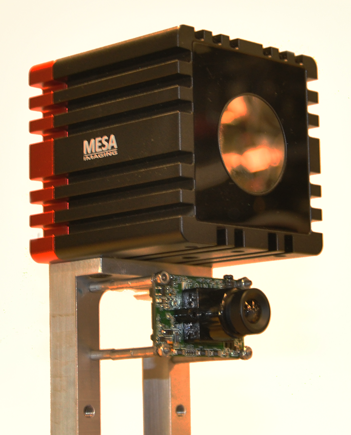
\includegraphics[width = 5cm]{camerasetup.png}
	\caption[SwissRanger depth camera and Firefly color camera setup]{SwissRanger depth 
		camera (top) and Firefly color camera (bottom) setup.}
	\label{camerassetup}
\end{figure}

Figure \ref{camerassetup} shows a setup of two camera sensors fixed on a frame, one below the other. The 
camera at the bottom is a Firefly, a Firewire camera manufactured by Point Grey \cite{FireflyDatasheet}. 
It captures grayscale images that can be converted to color using functions from the libdc1394 library
(see Section \ref{dc1394javaacquire}). The size of the images captured by a Firefly is $640 \times 480$ 
pixels.

The camera on top is a SwissRanger SR4000, a 3D time-of-flight camera manufactured by Mesa Imaging. 
It captures x-coordinate, y-coordinate, and z-coordinate information from the scene 
in front of the camera. This chapter focuses on the z-coordinate data, which will be referred to from this point 
on as the \textit{depth image}.\footnote{Similarly, the SwissRanger camera will also be referred to as the 
\textit{depth camera}.} The SwissRanger also produces an amplitude image, which corresponds to 
the amplitude of the modulated signal used in the depth measurements. The amplitude image can be used 
both for generating a grayscale image representing the captured scene and for measuring the quality of the 
depth values \cite{SR4000Manual}. The size of all images captured by the SwissRanger is $176 \times 144$
pixels.

Depending on the lens in the Firefly, the field of view of the color camera can be inside the field of view of the 
SwissRanger, or vice versa. Since the Firefly is more flexible in the matter of changing its field of view, this 
setup uses a wide angle lens on the color camera that makes it encompass the field of view of the depth 
camera. Figure \ref{imagetypes} shows an example of the three types of images captured by this 
depth-color camera setup. 
 

\begin{figure}[t]
	\center
	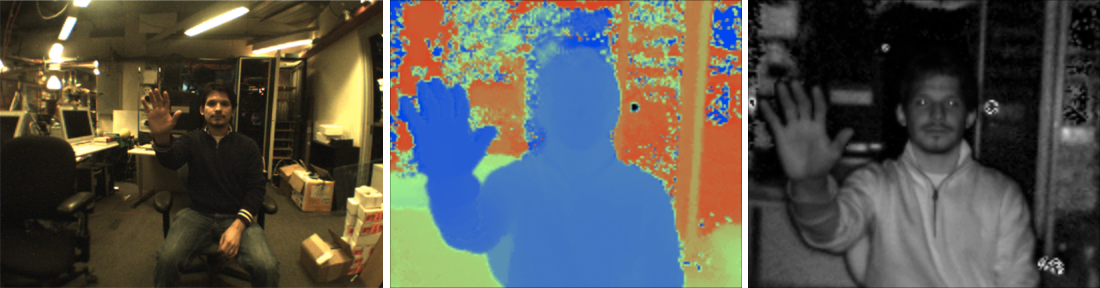
\includegraphics[width = 15cm]{data.png}
	\caption[Image types captured by the depth-color camera setup]{Image types captured by the 
		depth-color camera setup. From left to right: color image, depth image, and amplitude image.
		Notice the difference between the field of views of both cameras.}
	\label{imagetypes}
\end{figure}

\section{Fusion Algorithm} \label{algorithm}
The goal of the depth-color fusion algorithm is to find the correspondences between the pixels of a depth 
image and the pixels of a color image that have been acquired with a depth-color camera setup like the one 
described in Section \ref{cameras}. The first step of the algorithm is to retrieve the intrinsic and extrinsic 
parameters from both cameras. This is achieved by performing synchronized camera calibration. 

Given the cameras' parameters, the next step computes the relative transformation between the depth 
and color cameras, which is described in terms of a rotation and a translational offset. The relative 
transformation is used to transform world points in the depth camera's coordinate system to world points in
the color camera's coordinate system. The correspondences between points in the depth image and points 
in the color image are retrieved from an image point to world point transformation, followed by a world point 
to image point transformation.


\subsection{Cameras Calibration} \label{camerascalibration}


The depth and color cameras need to be calibrated in order to retrieve their intrinsic and extrinsic 
parameters. Since the goal is to find how the cameras are positioned and oriented one with respect to the 
other, the calibration of the cameras needs to be performed synchronously. In other words, there needs
to exist a positional correspondence between the calibration images taken with both cameras. This is 
achieved by setting the calibration pattern in a fixed position with respect to the camera setup and capturing 
one image from each camera at the same time. The two synchronized images are called an 
\textit{image pair} (see Figure \ref{imagepair}). 

\begin{figure}[t]
	\center
	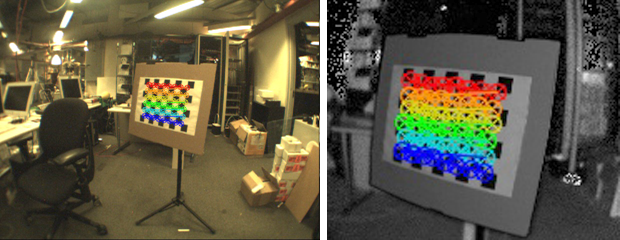
\includegraphics[width = 15cm]{imagepair.png}
	\caption[Example of a calibration image pair]{Example of a calibration image pair. An image pair is 
	composed of a color image (left) and an amplitude image from the depth camera (right).}
	\label{imagepair}
\end{figure}

As observed in Figure \ref{imagepair}, the image pair consists of a color image and an amplitude image. 
Since the amplitude image is visually similar to a grayscale image, it is possible to use it in the calibration 
process to find the calibration pattern. The colored circles in the figure indicate the location of the corners
in the pattern (see Section \ref{calibrationtool}). Besides knowing the correspondence between the images 
in an image pair, the synchronized calibration algorithm needs to know the correspondence between the 
calibration points in the two images.

The calibration process described in Section \ref{calibrationtool} computes the camera's focal length and 
principal point. If $f$ is the focal length of a camera, and $m_x$, $m_y$ are the ratios of pixel width and pixel 
height per unit distance, respectively, then $(f_x, f_y)$ represents the focal length expressed in units of 
horizontal and vertical pixels. That is, 
\begin{align}
(f_x, f_y) = ( f m_x , f m_y)
\end{align}

Furthermore, $(x_0, y_0)$ represents the principal point of the camera. Assuming that the skew coefficient 
between the $x$ and $y$ axes is zero, the intrinsic matrix of this camera is given by 
\begin{align} \label{intrinsicmatrix}
\mathbf{K} = \begin{bmatrix}
	f_x & 0    & x_0 \\
	0    & f_y & y_0 \\
	0    & 0    & 1      \\
\end{bmatrix}
\end{align}

The calibration process also provides a rotation matrix and a translation vector. These parameters describe
the transformation between the world's coordinate system and the camera's coordinate system. If 
$\mathbf{R}$ denotes the $3 \times 3$ rotation matrix, and $\mathbf{t}$ denotes the $3 \times 1$ 
translation vector, the extrinsic matrix of this camera is given by the $3 \times 4$ matrix 
\begin{align} \label{extrinsicmatrix}
\begin{bmatrix} \mathbf{R} & \mathbf{t} \\ \end{bmatrix}
\end{align}

Therefore, the synchronized calibration algorithm outputs two intrinsic matrices, $\mathbf{K}_d$ and 
$\mathbf{K}_c$, and two extrinsic matrices, $[ \mathbf{R}_d ~ \mathbf{t}_d ]$ and 
$[ \mathbf{R}_c ~ \mathbf{t}_c ]$, where the $d$ and $c$ subscripts are used to differentiate between the 
depth camera's parameters and the color camera's parameters. While the intrinsic matrices contain 
information about the internals of the camera, the extrinsic matrices hold information about how the 
cameras are positioned in space. This information is used in the next section to compute the relative 
transformation between both cameras. 


\subsection{Relative Transformation} \label{relativetransformation}


When computing the relative transformation between the cameras, the direction of the transformation is 
chosen to be from the depth camera to the color camera. As discussed in Section \ref{cameras}, the field
of view of the depth camera is within the field of view of the color camera. Therefore, every point in the depth
image will have a corresponding point in the color image, but not necessarily vice versa.

If $\mathbf{P} = (X, Y, Z)^T$ is a point in world coordinates, the position of $\mathbf{P}$ in the depth 
camera's coordinate system is given by $\mathbf{q}_d$. Similarly, the position of $\mathbf{P}$ in the color 
camera's coordinate system is given by $\mathbf{q}_c$. The points $\mathbf{q}_d$ and $\mathbf{q}_c$ 
can be expressed in terms of the cameras' extrinsic parameters by equations \eqref{qd} and \eqref{qc}, 
respectively.
\begin{align}
\mathbf{q}_d = \mathbf{R}_d \mathbf{P} + \mathbf{t}_d	\label{qd} \\
\mathbf{q}_c = \mathbf{R}_c \mathbf{P} + \mathbf{t}_c  	\label{qc}
\end{align}

Considering now the image of $\mathbf{P}$ in the depth image as having coordinates $(x_d, y_d)$, this
point can be expressed in homogeneous coordinates as $\mathbf{p}_d = (w x_d, w y_d, w )^T$, for some 
constant $w$. Using the depth camera's intrinsic parameters, $\mathbf{p}_d$ can be expressed by the 
equation:
\begin{align}
	\mathbf{p}_d = \mathbf{K}_d \mathbf{q}_d \label{pd}
\end{align}

This automatically reveals another expression for $\mathbf{q}_d$:
\begin{align}
	\mathbf{q}_d  = \mathbf{K}_{d}^{-1} \mathbf{p}_d \label{qd2}
\end{align}

Combining the two expressions for $\mathbf{q}_d$ (equations \eqref{qd} and \eqref{qd2}), and solving for 
$\mathbf{P}$ gives an equation for point $\mathbf{P}$:
\begin{align}
	\mathbf{K}_{d}^{-1} \mathbf{p}_d &= \mathbf{R}_d \mathbf{P} + \mathbf{t}_d \nonumber \\
	\mathbf{R}_d \mathbf{P} &= \mathbf{K}_{d}^{-1} \mathbf{p}_d - \mathbf{t}_d  \nonumber \\
	\mathbf{P} &= \mathbf{R}_{d}^{-1} \mathbf{K}_{d}^{-1} \mathbf{p}_d - \mathbf{R}_{d}^{-1} \mathbf{t}_d  
\end{align}

This expression for $\mathbf{P}$ can be substituted in equation \eqref{qc} to get a new expression for 
$\mathbf{q}_c$:
\begin{align}
	\mathbf{q}_c &= \mathbf{R}_c (\mathbf{R}_{d}^{-1} \mathbf{K}_{d}^{-1} \mathbf{p}_d 
					- \mathbf{R}_{d}^{-1} \mathbf{t}_d  ) + \mathbf{t}_c \nonumber \\
			    & =  \mathbf{R}_c \mathbf{R}_{d}^{-1} \mathbf{K}_{d}^{-1} \mathbf{p}_d
			    		 - \mathbf{R}_c \mathbf{R}_{d}^{-1} \mathbf{t}_d + \mathbf{t}_c \label{qc2}
\end{align}

Using equation \eqref{qd2}, equation \eqref{qc2} simplifies to:
\begin{align}
	\mathbf{q}_c &=  (\mathbf{R}_c \mathbf{R}_{d}^{-1}) ~ \mathbf{q}_{d}  
		+ (\mathbf{t}_c - \mathbf{R}_c \mathbf{R}_{d}^{-1} \mathbf{t}_d) \label{qc3}
\end{align}

Equation \eqref{qc3} reveals how the world points in the depth camera's coordinate system are related to 
the world points in the color camera's coordinate system. As seen from the equation, this
transformation is given in terms of the cameras' extrinsic parameters. Therefore, the relative transformation
between the depth and color cameras is defined by the rotation matrix in equation \eqref{relativerotation}
and the translation vector in equation \eqref{relativetranslation}.
\begin{align}
	\mathbf{R}_r = \mathbf{R}_c \mathbf{R}_{d}^{-1} \label{relativerotation} \\
	\mathbf{t}_r = \mathbf{t}_c - \mathbf{R}_r \mathbf{t}_d \label{relativetranslation}
\end{align}


\subsection{Point Correspondences} \label{pointcorrespondences}


The fusion algorithm must convert every point $(x_d, y_d)$ in the depth image into a point $(x_c, y_c)$ in 
the color image. This is achieved by first computing the world point $\mathbf{q}_d$ from the depth image
point $(x_d, y_d)$. Then, $\mathbf{q}_d$ is transformed into $\mathbf{q}_c$ using the results from Section 
\ref{relativetransformation}. Finally, world point $\mathbf{q}_c$ is converted into a color image point 
$(x_c, y_c)$.

If $(f_x, f_y)$ and $(x_0, y_0)$ are the focal length and principal point of the depth camera, respectively, 
the world point $\mathbf{q}_d = (X, Y, Z)^T$ can be related to the image point $(x_d, y_d)$ through the 
perspective projection equations \eqref{xd} and \eqref{yd}. 
\begin{align}
	x_d &= f_x \frac{X}{Z} + x_0 \label{xd} \\
	y_d &= f_y \frac{Y}{Z} + y_0 \label{yd} 
\end{align}
	
The depth camera provides the $z$-component of $\mathbf{q}_d$.\footnote{The depth camera can actually 
provide all components as discussed in Section \ref{cameras}. However, the noise in these measurements is 
high and recomputing the $x$ and $y$ components delivers better results.}
The $x$ and $y$ components are computed by solving equations \eqref{xd} and \eqref{yd} for $X$ and 
$Y$, respectively:
\begin{align}
	X = \frac{Z}{f_x} (x_d - x_0) \label{X} \\
	Y = \frac{Z}{f_y} (y_d - y_0) \label{Y}
\end{align}

Using the color camera's intrinsic parameters, $\mathbf{p}_c$ can be expressed by the equation
\begin{align}
	\mathbf{p}_c = \mathbf{K}_c \mathbf{q}_c \label{pc}
\end{align}

Furthermore, equation \eqref{qc3} gives an expression for $\mathbf{q}_c$. Therefore, combining 
\eqref{pc} and \eqref{qc3} results in a new equation for $\mathbf{p}_c$:
\begin{align}
	\mathbf{p}_c &=  \mathbf{K}_c (\mathbf{R}_r \mathbf{q}_{d}  + \mathbf{t}_r) \label{pc2}
\end{align}

By expressing $\mathbf{q}_{d}$ in homogeneous coordinates (that is, $\mathbf{q}_{d}^{'} = (X, Y, Z, 1)^T$), 
equation \eqref{pc2} can be rewritten as 
\begin{align}
	\mathbf{p}_c &=  \mathbf{K}_c [\mathbf{R}_r  ~  \mathbf{t}_r] \mathbf{q}_{d}^{'} \label{pc3}
\end{align}

The image coordinates $(x_c, y_c)$ are obtained by dividing the first and second components of 
$\mathbf{p}_c$ by its third component. That is, if $\mathbf{p}_c = (x,y,z)^T$, then 
\begin{align}
	(x_c, y_c) = \Bigg( \frac{x}{z} , \frac{y}{z} \Bigg) \label{xcyc}
\end{align}




\section{Implementation in the Vision System} \label{implementation}
	
The vision system described in Chapter \ref{system} provides the core structure needed to implement the 
depth-color fusion algorithm. The implementation is introduced in the form of a new camera object that 
provides fused depth-color images. The following sections discuss the classes that make up this 
representation, and the module dependency diagram in Figure \ref{depthcolorcammoduledependency} 
illustrates how they are related to the components of the vision system.

\begin{figure}[t]
\begin{center}
\digraph[scale=0.72]{DepthColorCam}{
	graph [rankdir = "TB" margin = 0];
	node [shape = "box" style = "filled" fillcolor = "gainsboro" fontsize = "12" fontname = "Courier"];
		Camera CameraData;
	node [shape = "box" style = "filled" fillcolor = "floralwhite" fontsize = "12" fontname = "Courier"];
	{ rank = "source"; Camera CameraData;}
	{ rank = "same"; DepthColorCam DepthColorCamData;}
	{ rank = "same"; ColorCam SwissRangerCam;}
	{ rank = "same"; DepthColorCalibrationTool DepthColorFusion;}
	{ rank = "sink"; CalibrationTool ;}
	edge [arrowhead = "normal"];
	Camera -> CameraData;
	DepthColorCam -> Camera [arrowhead = "empty"] ;
	DepthColorCam -> DepthColorCamData;
	DepthColorCam -> DepthColorCalibrationTool;
	DepthColorCam -> DepthColorFusion;
	DepthColorCam -> ColorCam;
	DepthColorCam -> SwissRangerCam;
	DepthColorCamData -> CameraData [arrowhead = "empty"];
	DepthColorCalibrationTool -> CalibrationTool;
	ColorCam -> CalibrationTool;
	SwissRangerCam -> CalibrationTool;
}
\caption[\DepthColorCam{}'s module dependency diagram]{\DepthColorCam{} module dependency diagram. 
Arcs with white arrows represent subtype relations (A $\vartriangleright$ B = A extends B) while arcs with 
black arrows represent implementation relations (A $\blacktriangleright$ B = A uses B). Gray rectangles 
represent abstract classes. The \ImageBuffer{} class is omitted from this diagram.}
\label{depthcolorcammoduledependency}
\end{center}
\end{figure}

	\subsection{Depth-Color Camera} \label{depthcolorcam}
	The \DepthColorCam{} class represents a camera that provides fused depth-color images. It extends the 
\Camera{} abstract class, the base camera representation discussed in Section \ref{camera}. The 
implementation of the \DepthColorCam{} class, however, differs from that of the \ColorCam{} and 
\SwissRangerCam{} classes (see Sections \ref{colorcam} and \ref{swissrangercam}). The principal reason for 
the difference comes from the fact that instead of representing an actual sensor device, this class represents 
the merging of a depth camera with a color camera through the algorithmic process discussed in Section 
\ref{algorithm}.

In order to respond to this representation, the \DepthColorCam{} class instantiates a \SwissRangerCam{} 
object and a \ColorCam{} object. As discussed before, this means the acquired depth and color images can
either come directly from the cameras or be transferred through the network. Before obtaining the fused 
images, the depth-color camera needs to be calibrated using the \DepthColorCalibrationTool{}. This 
calibration tool provides the cameras' parameters needed by the \DepthColorFusion{} class to fuse the 
acquired depth and color images.

Table \ref{depthcolorcammethods} lists the methods of the \DepthColorCam{} class. The depth-color camera
object provides access to the fused image through the \texttt{get\-Fused\-Col\-or} and \texttt{get\-Depth}
methods. The first method returns the image buffer containing the color information of the fused image. The
second method returns the image buffer containing the depth information. The camera object also provides
access to the original color image (\texttt{get\-O\-rig\-i\-nal\-Col\-or}) and to the amplitude image associated 
with the depth measurements (\texttt{get\-Am\-pli\-tude}).

\begin{table}[ht]
\caption{Public methods in the \DepthColorCam{} class}
\begin{center}
\begin{tabular}{| l |}
	\hline 
	\multicolumn{1}{| c |}{\DepthColorCam{}} \\
	\multicolumn{1}{| c |}{{\small \texttt{extends} \Camera{}}} \\
	\hline \hline
	\texttt{getFusedColor} \\
	\texttt{getDepth} \\
	\texttt{getAmplitude} \\
	\texttt{getOriginalColor} \\
	\texttt{getDepthDisplay} \\
	\texttt{getAmplitudeDisplay} \\
	\texttt{getFusedColorView} \\
	\texttt{getDepthView} \\
	\texttt{getAmplitudeView} \\
	\texttt{getOriginalColorView} \\
	\texttt{getFusionTool} \\
	\texttt{getCalibrationTool} \\
	\texttt{getModulationFrequency} \\
	\texttt{setCameraParameters} \\
	\texttt{setupDepthColorFusion} \\
	\hline
\end{tabular}
\end{center}
\label{depthcolorcammethods}
\end{table}

Like the \SwissRangerCam{} class, the depth-color camera provides image buffers with the color
visualizations of the depth and amplitude images. These visualizations are obtained through the 
\texttt{get\-Depth\-Dis\-play} and \texttt{get\-Am\-pli\-tude\-Dis\-play} methods. Furthermore, all image streams
(fused color, depth, amplitude, and original color) are displayed in \RD{} using the \ImageView{} objects that 
are associated with each image buffer.

The rest of the methods are used to retrieve the modulation frequency on which the SwissRanger camera is
operating, to gain access to the \DepthColorCalibrationTool{} and \DepthColorFusion{} objects associated
with the depth-color camera, and to setup the depth-color fusion object after the camera has been calibrated. 

When capturing the image stream from the depth and color cameras, it is important to make sure that the
pair of acquired images belongs to the same point in time. Since the camera devices are different, the time
response of their capturing mechanisms is not identical. Furthermore, the transfer of the images from the 
cameras to the computer running \RD{} also accounts for the time difference between the 
images.\footnote{For example, the computer's processor speed might affect the image transfer time.}

To solve this synchronization problem, the depth-color camera uses the version of the \texttt{grab\-Im\-age} 
method in the \ColorCam{} and \SwissRangerCam{} objects that takes as input the desired timestamp of the 
image that will be grabbed (see Sections \ref{colorcam} and \ref{swissrangercam}). By using this method it is
possible to retrieve the two images closest in time while taking into account the timestamp offset. Table 
\ref{depthcolorgrabimage} describes the algorithm used by the \texttt{grab\-Im\-age} method in the 
depth-color camera to retrieve the depth and color images and produce the fused image.

\begin{table}[ht]
\caption[Algorithm for the \texttt{grabImage} method in \DepthColorCam{}]{Algorithm for the 
\texttt{grabImage} method in \DepthColorCam{}. The method returns \texttt{true} if the image  
was grabbed successfully and \texttt{false} otherwise.}
\begin{center}
\begin{tabular}{ l l }
\hline
\multicolumn{2}{l}{\texttt{GRAB\_IMAGE :}} \\
1 & \texttt{Grab image from color camera;} \\
2 & \texttt{{\bf If} the image is grabbed successfully} \\
3 & \hspace{0.6cm} \texttt{\bf Then:} \\
4 & \hspace{1.2cm} \texttt{Grab image from SwissRanger camera using as} \\
-  & \hspace{1.8cm} \texttt{input the timestamp of the color image;} \\
5 & \hspace{1.2cm} \texttt{{\bf If} the image is grabbed successfully} \\
6 & \hspace{1.8cm} \texttt{\bf Then:} \\
7 & \hspace{2.4cm} \texttt{Fuse the color and depth images;} \\
8 & \hspace{2.4cm} \texttt{Return true;} \\
9 & \hspace{1.8cm} \texttt{\bf Else:} \\
10 & \hspace{2.4cm} \texttt{Return false;} \\
11 & \hspace{0.6cm}\texttt{\bf Else:} \\
12 & \hspace{1.2cm} \texttt{Return false;} \\
\hline
\end{tabular}
\end{center}
\label{depthcolorgrabimage}
\end{table}

Another problem that arises with the depth-color camera involves the noisy nature of the SwissRanger
images. As mentioned in Section \ref{pointcorrespondences}, the noisy values for the $x$ and $y$ 
coordinates provided by the SwissRanger camera are discarded and recalculated using equations \eqref{X} 
and \eqref{Y}. The depth values, however, cannot be recalculated. The noise from the depth data produces 
a fused color image like the one shown in Figure \ref{noise}. In order to reduce this noise, some depth 
values are discarded based on depth and amplitude thresholds. Points that are too close, points that are too 
far, and points with small amplitude value are discarded. This produces areas with no depth and color 
information in the final fused depth-color image. 

\begin{figure}[t]
\center
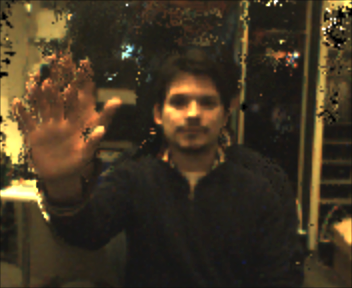
\includegraphics[scale = 0.5]{fusedcolornoise.png}
\caption{Fused color image without noise reduction}
\label{noise}
\end{figure}

Figure \ref{fusion} illustrates the result provided by the depth-color camera. It shows the original depth 
and color images, and next to them the fused color image. The black pixels in the depth and fused color
images indicate the points that were discarded due to data noise. It is worth noting that by thresholding the 
depth image it is possible to segment the object of interest from the background. 

\begin{figure}[t]
\center
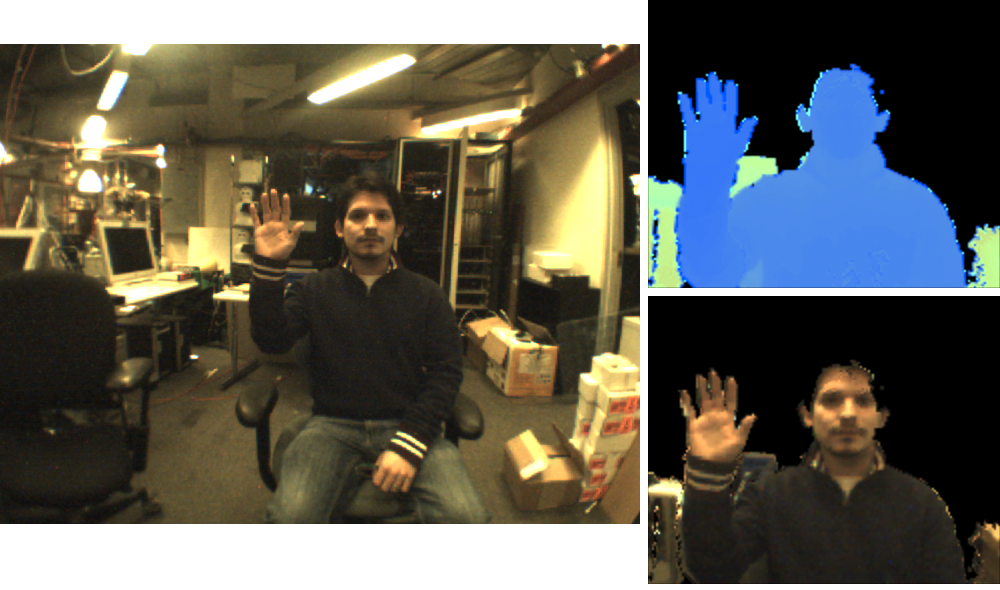
\includegraphics[width = 15cm]{fusion.png}
\caption[\DepthColorCam{}'s images]{\DepthColorCam{}'s images: the original color image (left), the 
depth image (upper right) and the fused color image (bottom right).}
\label{fusion}
\end{figure}



	
	\subsection{Depth-Color Calibration Tool} \label{depthcolorcalibrationtool}
	The \DepthColorCalibrationTool{} class implements the steps of the depth-color fusion algorithm that are 
described in Sections \ref{camerascalibration} and \ref{relativetransformation}. Analogous to the 
\DepthColorCam{} class, the implementation uses two \CalibrationTool{} objects, one for each of the cameras 
that is to be calibrated. The idea behind it consists of performing the calibration of both cameras in parallel, 
accepting an image pair only when the calibration pattern is found in both images.

Table \ref{depthcolorcalibrationtoolmethods} lists the methods of the \DepthColorCalibrationTool{} class. Similar
to a \CalibrationTool{} object, a depth-color calibration tool has methods to start, reset, and retrieve the status 
of the calibration process. It also provides methods to load and save the cameras' parameters, and to change
the default values of some of the parameters in the calibration process. 

\begin{table}[ht]
\caption{Public methods in the \DepthColorCalibrationTool{} class}
\begin{center}
\begin{tabular}{| l |}
	\hline 
	\multicolumn{1}{| c |}{\DepthColorCalibrationTool{}} \\
	\hline \hline
	\texttt{start} \\
	\texttt{reset} \\
	\texttt{isCalibrating} \\
	\texttt{calibrate} \\
	\texttt{setColorCameraParameters} \\
	\texttt{setDepthCameraParameters} \\
	\texttt{setChessboardSquareSize} \\
	\texttt{setChessboardDimensions} \\
	\texttt{setRequiredSamples} \\
	\texttt{getColorCameraParameters} \\
	\texttt{getDepthCameraParameters} \\
	\texttt{getChessboardNumberOfColumns} \\
	\texttt{getChessboardNumberOfRows} \\
	\texttt{getChessboardSquareSize} \\
	\texttt{getRequiredSamples} \\
	\texttt{getRelativeRotation} \\
	\texttt{getRelativeTranslation} \\
	\texttt{getRelativeTransformation} \\
	\texttt{loadCameraParameters} \\
	\texttt{saveCameraParameters} \\ 
	\hline
\end{tabular}
\end{center}
\label{depthcolorcalibrationtoolmethods}
\end{table}

The algorithm for the \texttt{cal\-i\-brate} method in the \DepthColorCalibrationTool{} class is also similar to the 
one seen in Section \ref{calibrationtool}. However, in this case it handles two calibration processes in parallel.
Throughout the steps of the algorithm described in Table \ref{depthcolorcalibratealgorithm}, the methods
\texttt{find\-And\-Draw\-Cor\-ners}, \texttt{add\-Cor\-ners\-To\-List}, and \texttt{cal\-i\-brate\-Cam\-er\-a}  
are called simultaneously on the two calibration tool objects used by the depth-color calibration tool.

\begin{table}[ht]
\caption{Algorithm for the \texttt{calibrate} method in \DepthColorCalibrationTool{}}
\begin{center}
\begin{tabular}{ l l }
\hline
\multicolumn{2}{l}{\texttt{CALIBRATE (currentImages, requiredImages):}} \\
1 & \texttt{{\bf If} (currentImages < requiredImages)} \\
2 & \hspace{0.6cm} \texttt{\bf Then:} \\
3 & \hspace{1.2cm} \texttt{Search checkerboard pattern in color image;} \\
4 & \hspace{1.2cm} \texttt{Search checkerboard pattern in amplitude image;} \\
5 & \hspace{1.2cm} \texttt{{\bf If} the pattern is found in both images} \\
6 & \hspace{1.8cm} \texttt{\bf Then:} \\
7 & \hspace{2.4cm} \texttt{Extract corners from color image and save them;} \\
8 & \hspace{2.4cm} \texttt{Extract corners from amplitude image and save them;} \\
9 & \hspace{2.4cm} \texttt{Increment currentImages counter;} \\
10 & \hspace{0.6cm} \texttt{\bf Else:} \\
11 & \hspace{1.2cm} \texttt{Run color camera calibration with saved corners;} \\
12 & \hspace{1.2cm} \texttt{Run depth camera calibration with saved corners;} \\
13 & \hspace{1.2cm} \texttt{Compute relative transformation with computed parameters;} \\
\hline
\end{tabular}
\end{center}
\label{depthcolorcalibratealgorithm}
\end{table}

This synchronized calibration takes advantage of the underlying OpenCV calibration functions. As mentioned in 
Section \ref{calibrationtool}, the calibration is performed using the functions in the OpenCV open source library. 
The function \texttt{cv\-Find\-Chess\-board\-Cor\-ners}, for example, locates the corners of a checkerboard 
(chessboard) pattern in an image \cite{Bradski}. Since it returns the corners ordered in row-major order 
starting from the upper-left corner, it is easy to know the correspondence between the calibration points 
in the depth image and the calibration points in the color image. 

As seen in Table \ref{depthcolorcalibratealgorithm}, the success of the calibration loop depends on finding the 
calibration pattern in both images of the image pair. When the calibration is completed for both
cameras, the relative transformation is calculated using equations \eqref{relativerotation} and 
\eqref{relativetranslation}. The parameters of the transformation can be accessed through three different 
methods. The \texttt{get\-Rel\-a\-tive\-Ro\-ta\-tion} and \texttt{get\-Rel\-a\-tive\-Trans\-la\-tion} methods return 
the $3 \times 3$ rotation matrix and $3 \times 1$ translation vector, respectively. The 
\texttt{get\-Rel\-a\-tive\-Trans\-for\-ma\-tion} method returns a $3 \times 4$ matrix in the form of an extrinsic 
matrix as described by equation \eqref{extrinsicmatrix}. Both the combination of the first two methods and the 
third method by itself provide all the necessary information to describe the transformation in 3D space between 
the depth camera and the color camera.

	
	\subsection{Depth-Color Fusion} \label{depthcolorfusion}
	The \DepthColorFusion{} class implements the steps of the depth-color fusion algorithm described in Section 
\ref{pointcorrespondences}. The constructor of this class takes as input the cameras' parameters 
computed with the \DepthColorCalibrationTool{} object. From these parameters it can calculate the relative 
transformation between the depth and color cameras using equations \eqref{relativerotation} and 
\eqref{relativetranslation}. Then, method \texttt{fuse\-Points}, listed in Table \ref{depthcolorfusionmethods},
can be used to get the point correspondences between the depth and color images.

\begin{table}[ht]
\caption{Public methods in the \DepthColorFusion{} class}
\begin{center}
\begin{tabular}{| l |}
	\hline 
	\multicolumn{1}{| c |}{\DepthColorFusion{}} \\
	\hline \hline
	\texttt{fusePoints} \\
	\texttt{getDepthCameraParameters} \\
	\texttt{getColorCameraParameters} \\
	\texttt{getDepthToColorMap} \\
	\texttt{getColorToDepthMap} \\
	\hline
\end{tabular}
\end{center}
\label{depthcolorfusionmethods}
\end{table}

Table \ref{fusepointsalgorithm} describes the algorithm for the \texttt{fuse\-Points} method. The method takes 
as input the depth image, the color image, and the image buffer where it will store the fused color information. 
For each pixel in the depth image it finds the correspondent pixel in the color image. Then, the algorithm 
retrieves the color value from the pixel in the color image and stores it in the pixel of the fused color buffer with 
position equal to the position of the depth image pixel. This fusion operation can be performed in real time with
live image streams.

\begin{table}[ht]
\caption{Algorithm for the \texttt{fusePoints} method in \DepthColorFusion{}}
\begin{center}
\begin{tabular}{ l l }
\hline
\multicolumn{2}{l}{\texttt{FUSE\_POINTS (depthImage, colorImage, fusedImage):}} \\
1 & \texttt{{\bf For} each pixel $(x_d, y_d)$ of depthImage:} \\
2 & \hspace{0.6cm} \texttt{Compute the world point $q_d$ using the depth value} \\
- & \hspace{1.2cm} \texttt{and equations \eqref{X} and \eqref{Y};} \\
3 & \hspace{0.6cm} \texttt{Compute homogeneous image point $p_c$ using equation \eqref{pc3};} \\
4 & \hspace{0.6cm} \texttt{Compute color image coordinate $(x_c, y_c)$ using equation \eqref{xcyc};} \\
5 & \hspace{0.6cm} \texttt{Retrieve color value from pixel $(x_c, y_c)$ of colorImage;} \\
6 & \hspace{0.6cm} \texttt{Place retrieved color value in pixel $(x_d, y_d)$ of fusedImage;} \\
\hline
\end{tabular}
\end{center}
\label{fusepointsalgorithm}
\end{table}

The final output of the depth-color fusion algorithm is a fused image that is composed of the original depth 
image and the fused color image. There is a one-to-one correspondence between the pixels of these images
with same $x$ and $y$ position. Furthermore, the \DepthColorFusion{} object stores the point correspondence
information in the form of two hash maps, one that maps points in the depth image to points in the original color
image, and another one that maps points in the original color image to points in the depth image. These hash
maps can be accessed through the \texttt{get\-Depth\-To\-Col\-or\-Map} and 
\texttt{get\-Col\-or\-To\-Depth\-Map} methods, respectively.






\chapter{Face and Body Pose Tracking} \label{applications}

Chapter \ref{system} presented an integrated vision system for \RD{}, and Chapter \ref{depthcolor} showed 
that it is possible to build new camera representations on top of it. Along with capturing and handling images, 
a vision system should be able to retrieve information from them. This chapter integrates two algorithms in the 
field of object detection and tracking that let the system gather information about humans in the 
camera's surroundings. 

Section \ref{facetracker} presents a face tracking algorithm that operates on the depth-color images introduced 
in Chapter \ref{depthcolor}. This algorithm uses the depth information to segment the person of interest from 
the background and consequently reduce the number of false positives detected by a traditional face detector.
The algorithm is shown to be robust to different face positions and orientations. 

Section \ref{bodyposetracker} introduces a representation for the Microsoft's Kinect camera and integrates an
open source framework that uses the Kinect's images to detect and track a person's body pose. The algorithm 
implemented in this framework operates on the depth images captured by the Kinect and outputs a body 
skeleton indicating the position and orientation of various joints in the human body. 

In this chapter, the Kinect becomes the second depth-color camera that forms part of the integrated vision 
system. In conjunction with the two tracking algorithms, this serves to point out the new importance of these 
sensors in the field of computer vision. 


\section{Face Tracker} \label{facetracker}
The images from a depth-color camera can be used to get better results from traditional face detection 
algorithms. The false positives from such algorithms come in part from pixels in the background that are 
thought to be faces. With the depth-color images, the depth information can be used to remove pixels from the 
background based on distance thresholds.

The \FaceTracker{} class implements an algorithm that uses the Viola-Jones object detection framework 
\cite{Viola} to find faces in depth-color images. Furthermore, after detecting the faces it uses the Camshift
(Continuously Adaptive Mean Shift) algorithm \cite{BradskiCamshift} to track them based on color information. 
The \FaceTracker{} uses the OpenCV library's implementations of the Viola-Jones and Camshift algorithms. 
\footnote{OpenCV implements the extended version of the Viola-Jones detector described by Lienhart and 
Maydt \cite{Lienhart}.}

The idea of the \FaceTracker{} algorithm consists of discarding the pixels in the fused color image that are
below or above certain depth thresholds. The value for these pixels are replaced with a zero value (a black 
pixel) creating uniform areas in the image that do not contain color information. Figure \ref{fusion} already
showed an example of a fused color image after thresholding based on depth. It revealed that this technique
can successfully segment the object of interest from the background, given that there is a significant distance
between the two.

Table \ref{facetrackeralgorithm} describes the algorithm of the \texttt{find\-Fac\-es} method, the main method 
of the face tracker class. This method performs the task of running the Viola-Jones detector and the Camshift 
tracker, and integrating the results from both algorithms.

\begin{table}[ht]
\caption{Algorithm for the \texttt{findFaces} method in \FaceTracker{}}
\begin{center}
\begin{tabular}{ l l }
\hline
\multicolumn{2}{l}{\texttt{FIND\_FACES (faceStream, successThreshold):}} \\
1 & \texttt{Run Viola-Jones face detector;} \\
2 & \texttt{{\bf If} face is detected} \\
3 & \hspace{0.6cm} \texttt{\bf Then:} \\
4 & \hspace{1.2cm} \texttt{Add face to faceStream;} \\
5 & \hspace{1.2cm} \texttt{{\bf If} the number of consecutive found faces} \\
- & \hspace{1.2cm} \texttt{is larger than successThreshold} \\
6 & \hspace{1.8cm} \texttt{\bf Then:} \\
7 & \hspace{2.4cm} \texttt{Initialize Camshift with the detection} \\
- & \hspace{2.4cm} \texttt{window of the found face} \\
8 & \hspace{0.6cm} \texttt{\bf Else:} \\
9 & \hspace{1.2cm} \texttt{{\bf If} faceStream contains a face for the last image} \\
- & \hspace{1.2cm} \texttt{and Camshift has been initialized} \\
10 & \hspace{1.8cm} \texttt{\bf Then:} \\
11 & \hspace{2.4cm} \texttt{Run the Camshift tracker;} \\
12 & \hspace{2.4cm} \texttt{{\bf If} face is successfully tracked} \\
13 & \hspace{3.0cm} \texttt{\bf Then:} \\
14 & \hspace{3.6cm} \texttt{Add face to faceStream;} \\
\hline
\end{tabular}
\end{center}
\label{facetrackeralgorithm}
\end{table}

The algorithm gives priority to the Viola-Jones detector over the Camshift tracker, mainly because Camshift 
only relies on tracking a patch of pixels with color distribution similar to that of a reference patch. Furthermore, 
this design follows the assumption that a person, the object of interest for the \FaceTracker{}, will be facing the 
camera most of the time, prompting in that way a high rate of successful face detections. Therefore, the 
detector is ran on every call to \texttt{find\-Fac\-es} (line 1), while the tracker is used as a backup for when the 
detector fails to find a face (line 11). 

The Camshift tracker needs to ``initialized'' before it can track a face (line 7). This initialization consists of 
building a histogram of the color information in a given reference window. The color information is the hue 
channel of the image and the reference window is the face detection window outputted by the Viola-Jones 
detector. Afterwards, every run of the tracker (line 11) calculates the back projection of the input image's hue 
channel using the reference histogram, and uses that to find the new location of the reference face. It is not
necessary to reinitialize the tracker on every successful detection because on consecutive image frames 
the position of the face does not change drastically. However, after some time the information in the reference
histogram might need to be refreshed, making necessary to reinitialize the tracker with a new face detection
window (lines 5 to 7).

The faces found by the \FaceTracker{} algorithm are added to a \FaceStream{} object (lines 4 and 14). The 
\FaceStream{} class extends \Stream{} and is similar in concept to the image stream representation discussed
in Section \ref{imagestream}. In this case, the stream uses objects of the type \List{} as buffer objects. In these 
lists the stream can store multiple instances of the \Face{} class, a simple data structure that holds the face's 
position and dimension. The advantage of storing the found faces in a face stream is that the user can 
define other algorithms based on the stored result of consecutive calls to \texttt{find\-Fac\-es}.

Table \ref{facetrackermethods} lists the methods of this class. The \texttt{de\-tect\-Fac\-es}, 
\texttt{in\-i\-tial\-ize\-Track\-ers}, and \texttt{track\-Fac\-es} methods are called by \texttt{find\-Fac\-es} to 
run the Viola-Jones detector, initialize Camshift, and run the Camshift tracker, respectively. The 
\texttt{get\-Fac\-es\-In\-Fused} method can be used to access the faces found on the last call to 
\texttt{find\-Fac\-es}. The actual face stream is accessed through the \texttt{get\-Fac\-es\-In\-Fused\-Stream} 
method.

\begin{table}[ht]
\caption{Public methods in the \FaceTracker{} class}
\begin{center}
\begin{tabular}{| l |}
	\hline 
	\multicolumn{1}{| c |}{\FaceTracker{}} \\
	\hline \hline
	\texttt{findFaces} \\
	\texttt{detectFaces} \\
	\texttt{initializeTrackers} \\
	\texttt{trackFaces} \\
	\texttt{mapFace} \\
	\texttt{getFacesInFused} \\
	\texttt{getFacesInColor} \\
	\texttt{getFacesInFusedStream} \\
	\texttt{getFacesInColorStream} \\
	\texttt{drawFaceInColor} \\
	\texttt{drawFaceInFused} \\
	\texttt{findFaceInterior} \\
	\texttt{mapFaceInterior} \\
	\hline
\end{tabular}
\end{center}
\label{facetrackermethods}
\end{table}

Furthermore, since the \DepthColorFusion{} object contains the mapping from pixels in the depth image to 
pixels in the color image (see Section \ref{depthcolorfusion}), it is possible to know the position of the face in 
the original color image. The \texttt{map\-Face} method is used to map faces from the fused color image to the 
original color image. This method is called automatically by the face tracker in order to provide an additional 
stream of faces. The \texttt{get\-Fac\-es\-In\-Col\-or} and \texttt{get\-Fac\-es\-In\-Col\-or\-Stream} methods
are used to access the faces in the original color image. 

The face tracker takes advantage of this mapping by providing the capability of detecting the 
eyes, nose, and mouth of a face using the Viola-Jones detector. Since the fused color image does not provide 
the necessary resolution to detect face parts, the face tracker uses the mapped face to run the detector 
on the region of interest of the original color image. The \texttt{find\-Face\-In\-te\-ri\-or} method performs this 
operation, and the \texttt{map\-Face\-In\-te\-ri\-or} method can be used to map the positions of the eyes, nose, 
and mouth back to the depth-color image.

Figure \ref{facetrackersequence} shows a sequence of fused color images that have passed through the
\FaceTracker{}'s algorithm. The red squares indicate the position and dimension of the face that was found 
on each of the images. Once the face tracker detects a person facing the camera, it can start tracking the face
through different head movements. The sequence of images shows that the algorithm is robust to change in 
face position (including distance from the camera) and orientation.

\begin{figure}[t]
\center
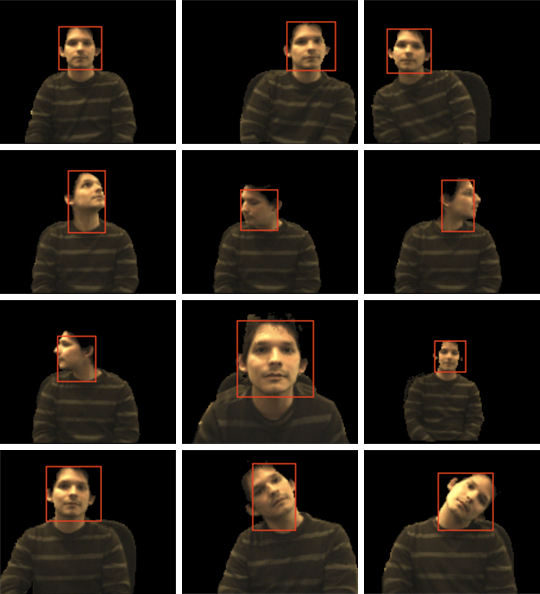
\includegraphics[width = 10cm]{facetracker.png}
\caption[Output of the \FaceTracker{}'s algorithm]{Output of the \FaceTracker{}'s algorithm on a sequence 
of depth-color images. The red squares indicate the position and dimension of the faces.}
\label{facetrackersequence}
\end{figure}


\section{Body Pose Tracker} \label{bodyposetracker}
The vision system also provides a way of tracking the body pose of a person. This is achieved through the
OpenNI open source framework, which provides support for detecting and tracking the body of a human 
in depth images \cite{OpenNI}. OpenNI achieves this by attempting to fit a skeleton on a potential human body. 
The information about the skeleton's joints is used to extract the position and orientation of the body.

The OpenNI module that contains the skeleton fitting capabilities is designed to work exclusively with 
PrimeSense derived sensors \cite{PrimeSensor, NITE}. An example of such sensor is the Microsoft's Kinect 
camera. Similar to the depth-color camera setup described in Chapter \ref{depthcolor}, the Kinect is designed
to capture depth and color images, everything on a single piece of hardware. The Kinect's images can be 
retrieved using the PrimeSense interface provided by OpenNI.

In order to take advantage of OpenNI's body tracking support, the vision system introduces the \KinectCam{} 
class. This class serves both as a representation of the Kinect camera and an interface to the OpenNI 
framework. The \KinectCam{} class is implemented following the same structure as the \ColorCam{} and 
\SwissRangerCam{} classes (see Sections \ref{colorcam} and \ref{swissrangercam}). The \KinectJavaAcquire{}
class establishes the Java interface to OpenNI and as such is used to retrieve the images and body 
skeleton information. The \KinectPacketHandler{} class receives image and skeleton data that is transferred 
over the network. The \KinectReceiver{} uses instances of the two previous classes to handle the data streams 
from the Kinect. A Kinect receiver is used by the \KinectCam{} class to gain access to the image and 
skeleton data. 

This design reveals that, in the \RD{} environment, the Kinect camera is seen not only as a sensor that 
provides depth and color images, but also as a sensor that provides body skeleton data for every image 
frame. The skeleton data is represented with an object of type \KinectSkeleton{}. This object contains the 
position and orientation of every joint in the body skeleton generated by OpenNI. The Kinect receiver handles
the skeleton objects using an instance of the \KinectSkeletonStream{} class, a subtype of \Stream{}. The 
\KinectSkeletonStream{} class represents a sequence of detected body poses, and its design is similar to the 
design of the \FaceStream{} class discussed in Section \ref{facetracker}.

Table \ref{kinectcammethods} lists the methods that the \KinectCam{} class adds to the base camera
representation. The \texttt{get\-Skel\-e\-tons} method further exemplifies the idea that in this system the Kinect
captures image and body skeleton data. The \texttt{cre\-ate\-Dis\-play} method is used to create a color 
visualization of the raw depth data, and the \texttt{thresh\-old} method serves to threshold the values of the
depth image.

\begin{table}[ht]
\caption{Public methods in the \KinectCam{} class}
\begin{center}
\begin{tabular}{| l |}
	\hline 
	\multicolumn{1}{| c |}{\KinectCam{}} \\
	\multicolumn{1}{| c |}{{\small \texttt{extends} \Camera{}}} \\
	\hline \hline
	\texttt{getColor} \\
	\texttt{getDepth} \\
	\texttt{getSkeletons} \\
	\texttt{getDepthDisplay} \\
	\texttt{getColorView} \\
	\texttt{getDepthView} \\
	\texttt{createDisplay} \\
	\texttt{threshold} \\
	\hline
\end{tabular}
\end{center}
\label{kinectcammethods}
\end{table}

Figure \ref{bodyposetrackersequence} shows a sequence of depth images captured with the Kinect camera
along with superimposed red skeletons that illustrate the output of OpenNI's body tracking algorithm. As it has 
been seen before, thresholding the image based on the depth values can segment the body of a person from 
the background assuming there is a significant distance between the two. The top left image shows the position
of the body that is required to calibrate and start the tracking algorithm. The other images show that the 
algorithm is robust to different body positions and orientations. 

One of the principal advantages of the body skeleton data is that it can be used as input to gesture recognition
algorithms. For example, the skeleton can provide information about the position of a person's arms with 
respect to the rest of the body. This information can be used to train algorithms that classify certain arm 
movements into gestures, making possible to recognize, for example, an arm waving, pointing, or reaching out. 

\begin{figure}[t]
\center
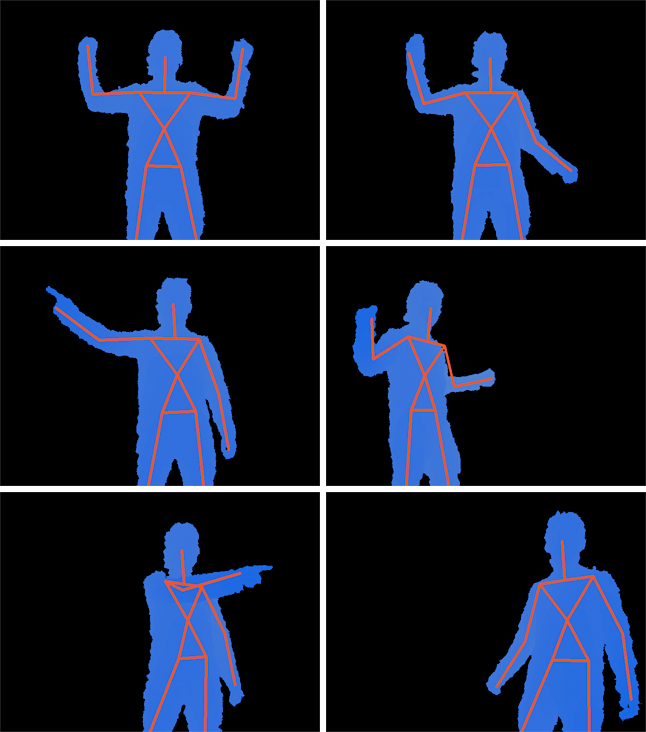
\includegraphics[width = 10cm]{bodyposetracker.png}
\caption[Output of OpenNI's body pose tracking algorithm]{Output of OpenNI's body pose tracking 
algorithm on a sequence of depth images. The red lines indicate the position of the skeleton's joints.}
\label{bodyposetrackersequence}
\end{figure}
\chapter{Conclusion} \label{conclusion}

This thesis presented an integrated vision system for a robotics research and development platform. The 
system was described as part of \RD{}, the software platform developed and used by the Personal Robots 
Group at the MIT Media Lab. Nevertheless, its design can be generalized and implemented in other platforms.

The proposed vision system featured representations for images and camera sensors. These representations
were shown to be versatile. For example, an \ImageBuffer{} can describe images of any size and with a variety 
of pixel depths and color models. Moreover, the \Camera{} and \CameraReceiver{} classes can be extended 
into subclasses that represent any type of camera. This thesis presented the implementations of three different 
types of cameras: a color camera, a 3D time-of-flight camera (or depth camera), and a Microsoft's Kinect 
camera.

Then, it was shown that it is possible to build new representations on top of the existing ones. The example 
discussed in this thesis was the \DepthColorCam{} class. The camera represented by this class merged the
representations of the depth and color cameras in order to provide images with fused depth-color information. 
To achieve this, it was necessary to describe an algorithm capable of performing the fusion of the depth and 
color images in real-time.

At the end, this thesis discussed two applications that use depth-color images to retrieve information from a 
scene. The first one used the images from the \DepthColorCam{} object to detect and track human faces. The
second application used the images from the Kinect, another depth-color camera, to detect and track human 
body pose. The algorithms that performed these operations proved to be robust to different positions and 
orientations of the face and body.

The system described in this thesis sets the basic requirements for the vision system of any robotics 
development platform. Color cameras have been the ``eyes'' of robots for many years. Now, depth-color 
cameras are becoming prime sensors in robotics. Robots like the MDS now have access to enhanced image 
data that can be used to design new computer vision algorithms with superior performance at retrieving
information about the robot's surroundings. 

Many joint efforts are involved in promoting the use of depth-color images in different applications. OpenNI is
led by industry leaders like PrimeSense and Willow Garage. The RGB-D Project \cite{RGBDProject}, a joint 
research effort between Intel Labs Seattle and the University of Washington, is another example of the 
potential these sensors have in future computer vision research.


\appendix
\chapter{Image Buffer Performance}

\begin{figure}[htbp]
\begin{center}
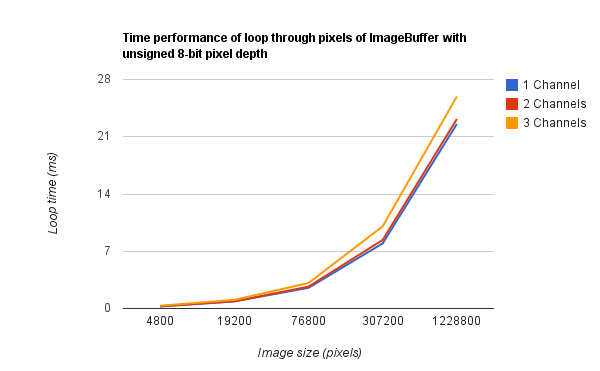
\includegraphics[scale = 0.75]{imagebufferlooptime.png}
\caption[Time performance of loop through all the pixels of an image buffer]{Time performance of loop through 
all the pixels of an image buffer. The tests were ran on image buffers of pixel depth \texttt{BYTE}, with 
one, two, and three channels. The tested image sizes were 80 x 60, 160 x 120, 320 x 240, 640 x 480, and 
1280 x 960.}
\end{center}
\end{figure}
\chapter{Depth-Color Fusion Performance}

\begin{figure}[htbp]
\begin{center}
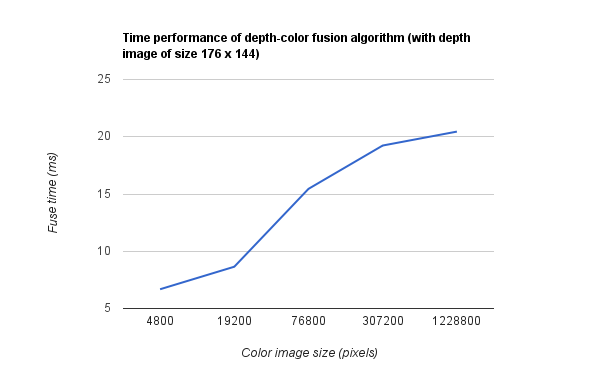
\includegraphics[scale = 0.75]{fusiontime.png}
\caption[Time performance of the depth-color fusion algorithm]{Time performance of the depth-color fusion 
algorithm. The tests were ran changing the size (resolution) of the color image while keeping the size of the 
depth image constant. The tested image sizes were 80 x 60, 160 x 120, 320 x 240, 640 x 480, and 
1280 x 960.}
\end{center}
\end{figure}

\begin{figure}[htbp]
\begin{center}
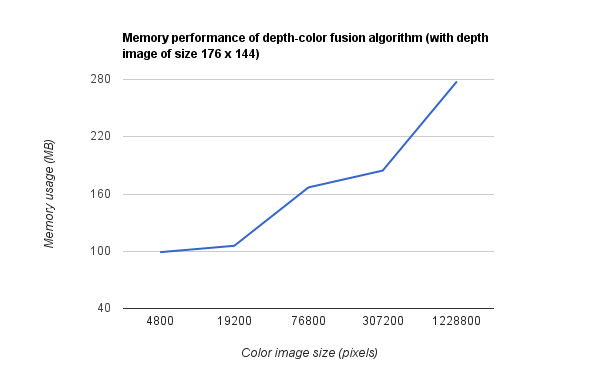
\includegraphics[scale = 0.75]{fusionmemory.png}
\caption[Memory performance of the depth-color fusion algorithm]{Memory performance of the depth-color 
fusion algorithm. The tests were ran changing the size (resolution) of the color image while keeping the size of 
the depth image constant. The tested image sizes were 80 x 60, 160 x 120, 320 x 240, 640 x 480, and 
1280 x 960.}
\end{center}
\end{figure}


\nocite{Horn}

%\appendix
%% This defines the bibliography file (main.bib) and the bibliography style.
%% If you want to create a bibliography file by hand, change the contents of
%% this file to a `thebibliography' environment.  For more information 
%% see section 4.3 of the LaTeX manual.
\begin{singlespace}
\bibliography{./content/main}
\bibliographystyle{content/IEEEtranS}
\end{singlespace}

	 
\end{document}